% !TEX program = xelatex
% !TeX TS-program = xelatex
% File này dùng fontspec (Times / TeX Gyre Termes) nên PHẢI biên dịch bằng
% XeLaTeX, không dùng pdfLaTeX. Ctrl+Alt+B sẽ đọc dòng !TEX ở trên.

\documentclass[12pt,a4paper]{report}

% ============================================================
% 1. FONT VÀ TIẾNG VIỆT - NÊN BIÊN DỊCH BẰNG XeLaTeX
% ============================================================
\usepackage{fontspec}
\usepackage{polyglossia}
\setmainlanguage{vietnamese}

% Ưu tiên Times New Roman nếu máy có.
% Nếu không có Times New Roman thì dùng TeX Gyre Termes (font gần giống Times).
% Nếu cũng không có thì dùng Latin Modern Roman.
\defaultfontfeatures{Mapping=tex-text}
\IfFontExistsTF{Times New Roman}{%
  \setmainfont{Times New Roman}%
}{%
  \IfFontExistsTF{TeX Gyre Termes}{%
    \setmainfont{TeX Gyre Termes}%
  }{%
    \setmainfont{Latin Modern Roman}%
  }%
}

% ============================================================
% 2. ĐỊNH DẠNG TRANG, GIÃN DÒNG, THỤT ĐẦU DÒNG
% ============================================================
\usepackage[left=3cm,right=2cm,top=2.5cm,bottom=2.5cm]{geometry}
\usepackage{setspace}
\usepackage{indentfirst}

\onehalfspacing
\setlength{\parindent}{1cm}
\setlength{\parskip}{0pt}

% ============================================================
% 3. CÁC GÓI HỖ TRỢ HÌNH ẢNH, BẢNG, CHÚ THÍCH, LIÊN KẾT
% ============================================================
% Không dùng [demo] — chế độ đó vẽ hình đen đặc.
\usepackage{graphicx}
\graphicspath{{images/}}

\usepackage{caption}
\usepackage{booktabs}
\usepackage{array}
\usepackage{tabularx}
\usepackage{longtable}
\usepackage{multirow}
\usepackage{amsmath}
\usepackage{float}
\usepackage{underscore}
\usepackage{tocloft}
\usepackage{titlesec}
\usepackage{tikz}
\usetikzlibrary{arrows.meta,positioning,shapes.geometric,fit,calc,shadows,shapes.multipart}
\usepackage{pgfplots}
\pgfplotsset{compat=1.18}
\usepackage[hidelinks]{hyperref}
\usepackage{xurl}

% Caption của bảng nằm phía trên bảng.
% Caption của hình nằm phía dưới hình.
\captionsetup[table]{
  position=above,
  skip=6pt,
  justification=centering,
  labelfont=bf,
  font=small
}

\captionsetup[figure]{
  position=below,
  skip=6pt,
  justification=centering,
  labelfont=bf,
  font=small
}

% ============================================================
% 4. ĐÁNH SỐ CÔNG THỨC, HÌNH, BẢNG THEO CHƯƠNG
% Ví dụ: Hình 2.1, Bảng 3.2, Công thức (2.1)
% ============================================================
\numberwithin{equation}{chapter}
\numberwithin{figure}{chapter}
\numberwithin{table}{chapter}

% ============================================================
% 5. TÊN CÁC PHẦN BẰNG TIẾNG VIỆT
% ============================================================
\AtBeginDocument{%
  \renewcommand{\chaptername}{Chương}
  \renewcommand{\contentsname}{MỤC LỤC}
  \renewcommand{\listfigurename}{DANH MỤC HÌNH VẼ}
  \renewcommand{\listtablename}{DANH MỤC BẢNG}
  \renewcommand{\bibname}{TÀI LIỆU THAM KHẢO}
  \renewcommand{\figurename}{Hình}
  \renewcommand{\tablename}{Bảng}
}

% ============================================================
% 6. ĐỊNH DẠNG CHƯƠNG, MỤC, MỤC LỤC
% ============================================================
\setcounter{secnumdepth}{3}
\setcounter{tocdepth}{3}

% Chương hiển thị dạng:
% Chương 1. TỔNG QUAN ĐỀ TÀI
\titleformat{\chapter}[block]
  {\normalfont\Large\bfseries\centering}
  {\chaptertitlename\ \thechapter.}{0.5em}{\MakeUppercase}
\titlespacing*{\chapter}{0pt}{0pt}{20pt}

% Section, subsection, subsubsection
\titleformat{\section}
  {\normalfont\bfseries}
  {\thesection}{0.6em}{}

\titleformat{\subsection}
  {\normalfont\bfseries}
  {\thesubsection}{0.6em}{}

\titleformat{\subsubsection}
  {\normalfont\bfseries\itshape}
  {\thesubsubsection}{0.6em}{}

% Thêm dấu chấm trong mục lục cho cấp chapter
\renewcommand{\cftchapdotsep}{\cftdotsep}
\renewcommand{\cftchapfont}{\normalsize\bfseries}

% ============================================================
% 7. THÔNG TIN CÁ NHÂN - THAY PHẦN NÀY
% ============================================================
\newcommand{\tenSV}{Lê Gia Bảo}
\newcommand{\maSV}{2351010016}
\newcommand{\tenDoAn}{XÂY DỰNG HỆ THỐNG TRỢ LÝ PHÁP LÝ AI CHO DOANH NGHIỆP NHỎ VÀ VỪA}
\newcommand{\tenNganh}{CÔNG NGHỆ THÔNG TIN}
\newcommand{\loaiBaoCao}{ĐỒ ÁN NGÀNH}
\newcommand{\namBaoCao}{2026}
\newcommand{\gvhd}{ThS. Dương Hữu Thành}
\newcommand{\gvhdInHoa}{ThS. DƯƠNG HỮU THÀNH}

% Khung viền kép + bố cục bìa theo mẫu khóa luận Trường ĐH Mở TP.HCM.
\newcommand{\khungBiaKep}{%
  \begin{tikzpicture}[remember picture, overlay]
    \draw[line width=2.4pt]
      ([xshift=1.05cm,yshift=-1.05cm]current page.north west)
      rectangle
      ([xshift=-1.05cm,yshift=1.05cm]current page.south east);
    \draw[line width=0.7pt]
      ([xshift=1.22cm,yshift=-1.22cm]current page.north west)
      rectangle
      ([xshift=-1.22cm,yshift=1.22cm]current page.south east);
  \end{tikzpicture}%
}

\newcommand{\trangBiaMau}{%
  \thispagestyle{empty}%
  \khungBiaKep
  \vspace*{-0.15cm}
  \begin{center}
    \singlespacing
    {\bfseries BỘ GIÁO DỤC VÀ ĐÀO TẠO\par}
    \vspace{4pt}
    {\bfseries TRƯỜNG ĐẠI HỌC MỞ THÀNH PHỐ HỒ CHÍ MINH\par}

    \vspace{0.7cm}
    
\includegraphics[height=2.55cm]{logo-ouhcmc.png}

    \vspace{1.15cm}
    {\Large\bfseries \tenDoAn\par}

    \vspace{1.45cm}
    \begin{tabular}{@{}p{5.8cm}@{\hspace{1.8cm}}r@{}}
      \textbf{\tenSV} & \textbf{\maSV}
    \end{tabular}

    \vspace{1.15cm}
    Giảng viên hướng dẫn: \textbf{\gvhdInHoa}

    \vfill
    {\large\bfseries \loaiBaoCao\par}
    \vspace{0.4cm}
    {\large\bfseries NGÀNH \tenNganh\par}

    \vspace{1.4cm}
    {\bfseries TP. HỒ CHÍ MINH, \namBaoCao\par}
    \vspace{0.15cm}
  \end{center}
}

% Số liệu về corpus. Khai báo một chỗ để mọi chương dùng chung,
% cập nhật ở đây khi corpus thay đổi.
\newcommand{\soLuat}{38}
\newcommand{\soDieu}{3.844}
\newcommand{\soChuong}{452}
\newcommand{\soRule}{12}
\newcommand{\soTest}{77}

% Khung trình bày kỹ thuật/công nghệ: Là gì / Vì sao / Cách dùng / Khi nào.
\newcommand{\boncau}[4]{%
\begin{itemize}
    \item \textbf{Là gì.} #1
    \item \textbf{Vì sao dùng.} #2
    \item \textbf{Cách dùng.} #3
    \item \textbf{Khi nào.} #4
\end{itemize}
}

% Các sơ đồ TikZ dùng chung — thay cho ảnh PNG đen (demo graphicx).
% Gọi bằng \hinhKienTruc, \hinhUseCase, ... trong môi trường figure.

\newcommand{\hinhKienTruc}{%
\begin{tikzpicture}[
  font=\footnotesize,
  box/.style={draw=black!70, rounded corners=2pt, align=center,
    minimum height=1.1cm, minimum width=2.6cm, fill=blue!6},
  arr/.style={-{Latex}, thick}
]
\node[box] (browser) at (0,3.2) {Trình duyệt\\React SPA};
\node[box, fill=green!8] (nginx) at (4.2,3.2) {nginx\\static + proxy \texttt{/api}};
\node[box, fill=orange!10] (api) at (4.2,1.2) {FastAPI\\REST + SSE};
\node[box, fill=yellow!15] (pg) at (0,1.2) {PostgreSQL 17\\FTS + nghiệp vụ};
\node[box, fill=purple!8] (chroma) at (8.0,1.2) {Chroma\\vector Điều};
\node[box, fill=red!6] (gemini) at (8.0,3.2) {Gemini API\\LLM + embedding};
\draw[arr] (browser) -- (nginx);
\draw[arr] (nginx) -- (api);
\draw[arr] (api) -- (pg);
\draw[arr] (api) -- (chroma);
\draw[arr] (api) -- (gemini);
\end{tikzpicture}%
}

\newcommand{\hinhUseCase}{%
\begin{tikzpicture}[
  font=\scriptsize,
  actor/.style={draw, ellipse, align=center, minimum width=1.8cm, minimum height=0.9cm},
  uc/.style={draw, rounded corners=2pt, align=center, minimum width=3.4cm,
    minimum height=0.55cm, fill=blue!4},
  sys/.style={draw=black!60, dashed, inner sep=8pt}
]
\node[actor] (guest) at (0,4.5) {Khách};
\node[actor] (owner) at (0,2.8) {Chủ DN};
\node[actor] (acc) at (0,1.2) {Kế toán\\/ Nhân sự};
\node[actor] (admin) at (0,-0.4) {Quản trị};

\begin{scope}[local bounding box=sysbox]
\node[uc] (uc01) at (5.2,5.0) {UC-01 Đăng ký};
\node[uc] (uc02) at (5.2,4.3) {UC-02 Đăng nhập};
\node[uc] (uc03) at (5.2,3.4) {UC-03 Hỏi đáp};
\node[uc] (uc05) at (5.2,2.7) {UC-05 Tra cứu luật};
\node[uc] (uc07) at (5.2,2.0) {UC-07 Soát hợp đồng};
\node[uc] (uc09) at (5.2,1.3) {UC-09 Lịch tuân thủ};
\node[uc] (uc10) at (5.2,0.4) {UC-10 Quản trị corpus};
\node[uc] (uc12) at (5.2,-0.3) {UC-12 Hàng loạt câu hỏi};
\end{scope}
\node[sys, fit=(uc01)(uc12), label=above:{\small Hệ thống trợ lý pháp lý}] {};

\draw (guest) -- (uc01); \draw (guest) -- (uc02);
\draw (owner) -- (uc03); \draw (owner) -- (uc05);
\draw (owner) -- (uc07); \draw (owner) -- (uc09);
\draw (acc) -- (uc03); \draw (acc) -- (uc05);
\draw (acc) -- (uc07); \draw (acc) -- (uc09);
\draw (admin) -- (uc10); \draw (admin) -- (uc12);
\draw (admin) -- (uc03);
\end{tikzpicture}%
}

\newcommand{\hinhRag}{%
\begin{tikzpicture}[
  font=\scriptsize,
  n/.style={draw, rounded corners=2pt, align=center, minimum width=2.3cm,
    minimum height=0.7cm, fill=blue!5},
  d/.style={-{Latex}, thick},
  skip/.style={-{Latex}, thick, red!60!black}
]
\node[n] (a) at (0,0) {analyze\_intent};
\node[n] (b) at (3.0,0) {prepare\_query};
\node[n] (c) at (6.0,0) {retrieve};
\node[n] (d) at (9.0,0) {rerank\\(tắt)};
\node[n] (e) at (3.0,-1.6) {llm\_filter};
\node[n] (f) at (6.0,-1.6) {generate};
\node[n] (g) at (9.0,-1.6) {format\_\\submission};
\node[n, fill=red!8] (skip) at (0,-1.6) {SKIP / hết};
\draw[d] (a) -- (b); \draw[d] (b) -- (c); \draw[d] (c) -- (d);
\draw[d] (d) |- (e); \draw[d] (e) -- (f); \draw[d] (f) -- (g);
\draw[skip] (a) -- (skip);
\end{tikzpicture}%
}

\newcommand{\hinhLop}{%
\begin{tikzpicture}[
  font=\footnotesize,
  layer/.style={draw, rounded corners=3pt, align=center, minimum height=1.35cm,
    minimum width=11.2cm},
]
\node[layer, fill=cyan!10] (ui) at (0,3.6)
  {\textbf{Lớp trình bày:} React 19 + Vite + TanStack Query + Zustand + Tailwind};
\node[layer, fill=orange!12] (app) at (0,1.8)
  {\textbf{Lớp ứng dụng:} FastAPI routers (auth, chat, laws, documents,\\
   compliance, admin, lab) + LangGraph agent + BackgroundTasks};
\node[layer, fill=green!10] (data) at (0,0)
  {\textbf{Lớp dữ liệu:} PostgreSQL (nghiệp vụ + FTS) · Chroma (vector) · BM25 RAM};
\draw[-{Latex}, thick] (ui) -- (app);
\draw[-{Latex}, thick] (app) -- (data);
\end{tikzpicture}%
}

\newcommand{\hinhCsdl}{%
\begin{tikzpicture}[
  font=\tiny,
  >=Latex,
  every node/.append style={font=\tiny},
  ent/.style={
    draw=black!75, very thin,
    rectangle split, rectangle split parts=2,
    rectangle split part align=left,
    align=left, inner sep=2.4pt,
    text width=3.28cm,
    font=\fontsize{5.6}{6.7}\selectfont\ttfamily
  },
  rel/.style={-{Latex}, thick, black!65},
  reld/.style={-{Latex}, thick, dashed, black!55},
  card/.style={font=\fontsize{5.4}{6.4}\selectfont, fill=white, inner sep=0.6pt}
]
% Hàng 1 --- tài khoản và hội thoại
\node[ent, rectangle split part fill={yellow!28,yellow!6}] (org) at (0,0)
  {\nodepart{one}\textbf{organizations}
   \nodepart{two}PK id uuid\\
   name\\
   tax\_code UK\\
   employee\_count\\
   vat\_period\\
   annual\_revenue\_bn};
\node[ent, rectangle split part fill={yellow!28,yellow!6}] (user) at (4.05,0)
  {\nodepart{one}\textbf{users}
   \nodepart{two}PK id uuid\\
   email UK\\
   password\_hash\\
   full\_name\\
   role, is\_active\\
   FK organization\_id};
\node[ent, rectangle split part fill={blue!22,blue!5}] (conv) at (8.10,0)
  {\nodepart{one}\textbf{conversations}
   \nodepart{two}PK id uuid\\
   FK user\_id\\
   title\\
   archived\\
   message\_count};
\node[ent, rectangle split part fill={blue!22,blue!5}] (msg) at (12.15,0)
  {\nodepart{one}\textbf{messages}
   \nodepart{two}PK id uuid\\
   seq Identity\\
   FK conversation\_id\\
   role, content\\
   citations JSONB\\
   trace JSONB};

% Hàng 2 --- hợp đồng và nhật ký
\node[ent, rectangle split part fill={teal!28,teal!6}] (doc) at (0,-4.15)
  {\nodepart{one}\textbf{documents}
   \nodepart{two}PK id uuid\\
   FK organization\_id\\
   FK uploaded\_by\\
   filename, mime\_type\\
   storage\_path\\
   status, extracted\_text};
\node[ent, rectangle split part fill={teal!28,teal!6}] (rev) at (4.05,-4.15)
  {\nodepart{one}\textbf{contract\_reviews}
   \nodepart{two}PK id uuid\\
   FK document\_id\\
   status\\
   risk\_score 0--100\\
   summary\\
   clause\_count};
\node[ent, rectangle split part fill={teal!28,teal!6}] (find) at (8.10,-4.15)
  {\nodepart{one}\textbf{contract\_findings}
   \nodepart{two}PK id uuid\\
   FK review\_id\\
   position\\
   clause\_text\\
   risk\_level\\
   legal\_refs JSONB};
\node[ent, rectangle split part fill={black!12,black!3}] (audit) at (12.15,-4.15)
  {\nodepart{one}\textbf{audit\_logs}
   \nodepart{two}PK id uuid\\
   FK user\_id SET NULL\\
   actor\_email\\
   action, resource\\
   resource\_id\\
   detail JSONB};

% Hàng 3 --- lịch tuân thủ và corpus
\node[ent, rectangle split part fill={orange!30,orange!7}] (rule) at (0,-8.35)
  {\nodepart{one}\textbf{compliance\_rules}
   \nodepart{two}PK id serial\\
   code UK\\
   frequency, due\_day\\
   legal\_refs JSONB\\
   applies\_to JSONB\\
   is\_active};
\node[ent, rectangle split part fill={orange!30,orange!7}] (task) at (4.05,-8.35)
  {\nodepart{one}\textbf{compliance\_tasks}
   \nodepart{two}PK id uuid\\
   FK organization\_id\\
   FK rule\_id\\
   period\_label\\
   due\_date, status\\
   UK (org, rule, kỳ)};
\node[ent, rectangle split part fill={green!28,green!6}] (laws) at (8.10,-8.35)
  {\nodepart{one}\textbf{laws}
   \nodepart{two}PK law\_id\\
   law\_name, doc\_type\\
   category\\
   article\_count\\
   status};
\node[ent, rectangle split part fill={green!28,green!6}] (lkr) at (12.15,-8.35)
  {\nodepart{one}\textbf{legal\_knowledge\_records}
   \nodepart{two}PK id (từ JSON)\\
   law\_id, article\\
   content, extra JSONB\\
   article\_number *\\
   search\_vector *};

% Quan hệ 1 -- N
\draw[rel] (org) -- node[card, above]{1} node[card, below]{N} (user);
\draw[rel] (user) -- node[card, above]{1} node[card, below]{N} (conv);
\draw[rel] (conv) -- node[card, above]{1} node[card, below]{N} (msg);
\draw[rel] (org) -- node[card, left]{1} node[card, right]{N} (doc);
\draw[rel] (doc) -- node[card, above]{1} node[card, below]{N} (rev);
\draw[rel] (rev) -- node[card, above]{1} node[card, below]{N} (find);
\draw[rel] (rule) -- node[card, above]{1} node[card, below]{N} (task);
\draw[rel] (org.south west) -- ++(-0.45,0) |- node[card, near start, left]{1} node[card, near end, left]{N} (task.west);
\draw[rel] (user.south east) -- ++(0.35,0) |- node[card, pos=0.15, right]{1} node[card, pos=0.72, right]{N} (audit.north);
\draw[reld] (user.south) -- node[card, left]{1} node[card, right]{N} (doc.north east);
\draw[reld] (laws) -- node[card, above]{1} node[card, below]{N} (lkr);

\node[anchor=west, font=\fontsize{5.6}{6.8}\selectfont, align=left] at (-1.75,-11.15) {%
  Nét liền: khóa ngoại thật (CASCADE hoặc SET NULL).
  Nét đứt: \texttt{uploaded\_by} và \texttt{laws}$\leftrightarrow$\texttt{legal\_knowledge\_records} (cùng \texttt{law\_id}, không FK).\\
  * = cột generated (Postgres tự tính).
  UK = unique.
  Màu: vàng tài khoản, xanh dương hội thoại, teal hợp đồng, cam lịch, xanh lục corpus, xám nhật ký.%
};
\end{tikzpicture}%
}

\newcommand{\hinhChatSeq}{%
\begin{tikzpicture}[
  font=\scriptsize,
  actor/.style={align=center},
  msg/.style={-{Latex}, thick}
]
\node[actor] (u) at (0,0) {Trình duyệt};
\node[actor] (a) at (4.2,0) {API};
\node[actor] (g) at (8.4,0) {LangGraph};
\draw (u) -- ++(0,-5.2); \draw (a) -- ++(0,-5.2); \draw (g) -- ++(0,-5.2);
\draw[msg] (0,-0.5) -- node[above,font=\tiny]{POST /chat/stream} (4.2,-0.5);
\draw[msg] (4.2,-1.1) -- node[above,font=\tiny]{INSERT câu hỏi} (4.2,-1.1);
\node[font=\tiny,anchor=west] at (4.4,-1.1) {ghi DB};
\draw[msg] (4.2,-1.8) -- node[above,font=\tiny]{chạy graph} (8.4,-1.8);
\draw[msg] (8.4,-2.5) -- node[above,font=\tiny]{SSE status/token} (0,-2.5);
\draw[msg] (8.4,-3.3) -- node[above,font=\tiny]{result} (4.2,-3.3);
\draw[msg] (4.2,-4.0) -- node[above,font=\tiny]{INSERT câu trả lời} (4.2,-4.0);
\node[font=\tiny,anchor=west] at (4.4,-4.0) {session mới};
\draw[msg] (4.2,-4.7) -- node[above,font=\tiny]{SSE result} (0,-4.7);
\end{tikzpicture}%
}

\newcommand{\hinhHopDongSeq}{%
\begin{tikzpicture}[
  font=\scriptsize,
  n/.style={draw, rounded corners=2pt, align=center, minimum width=2.1cm,
    minimum height=0.65cm, fill=teal!8},
  d/.style={-{Latex}, thick}
]
\node[n] (u) {Upload file};
\node[n, right=0.5cm of u] (e) {Trích chữ};
\node[n, right=0.5cm of e] (r) {ready};
\node[n, right=0.5cm of r] (p) {POST review\\202};
\node[n, below=0.7cm of p] (bg) {Background:\\cắt khoản + RAG};
\node[n, left=0.5cm of bg] (d) {done / failed};
\node[n, left=0.5cm of d] (ui) {UI poll 2,5s};
\draw[d] (u)--(e)--(r)--(p);
\draw[d] (p)--(bg)--(d)--(ui);
\end{tikzpicture}%
}

\newcommand{\hinhTrangThai}{%
\begin{tikzpicture}[
  font=\footnotesize,
  s/.style={draw, rounded corners=2pt, minimum width=2.0cm, minimum height=0.7cm,
    align=center, fill=gray!10},
  d/.style={-{Latex}, thick}
]
\node[s] (p) {pending};
\node[s, fill=blue!12, right=0.6cm of p] (r) {ready};
\node[s, fill=orange!15, right=0.6cm of r] (x) {processing};
\node[s, fill=green!15, right=0.6cm of x] (d) {done};
\node[s, fill=red!12, below=0.7cm of x] (f) {failed};
\draw[d] (p)--(r)--(x)--(d);
\draw[d] (x)--(f);
\draw[d, dashed] (f)|-(r);
\end{tikzpicture}%
}


\begin{document}

% Không đánh số trang ở hai trang bìa
\pagenumbering{gobble}
\newgeometry{left=2.2cm,right=2.2cm,top=1.65cm,bottom=1.65cm}

% ============================================================
% TRANG BÌA 1 và BÌA 2 (bố cục mẫu Trường ĐH Mở TP.HCM)
% ============================================================
\begin{titlepage}
\trangBiaMau
\end{titlepage}

\clearpage

\begin{titlepage}
\trangBiaMau
\end{titlepage}

\clearpage
\restoregeometry

% Bắt đầu đánh số La Mã cho phần đầu báo cáo
\pagenumbering{Roman}
\setcounter{page}{1}
\pagestyle{plain}

% ============================================================
% LỜI CẢM ƠN (giữ trang, không in nội dung)
% ============================================================
\chapter*{LỜI CẢM ƠN}
\addcontentsline{toc}{chapter}{LỜI CẢM ƠN}

Em xin gửi lời cảm ơn đến Thầy \gvhd{}, giảng viên hướng dẫn đồ án. Thầy đã
góp ý sớm về phạm vi đề tài, về việc hệ thống phải chạy được khi thiếu khóa mô
hình, và về việc mọi căn cứ trên giao diện phải mở được về Điều gốc. Những góp
ý đó định hình cách em thiết kế hàng rào dẫn chiếu và cách đóng gói Docker.

Em cảm ơn quý Thầy Cô Khoa Công nghệ thông tin, Trường Đại học Mở Thành phố Hồ
Chí Minh, đã giảng dạy các học phần nền để em đủ sức hoàn thành đồ án ngành.

Em cảm ơn gia đình đã tạo điều kiện học tập. Mọi thiếu sót trong báo cáo và
trong mã nguồn thuộc về em.

\begin{flushright}
\textit{Thành phố Hồ Chí Minh, năm \namBaoCao}\\[0.6em]
\textit{\tenSV}
\end{flushright}

\clearpage

\chapter*{NHẬN XÉT CỦA GIÁO VIÊN HƯỚNG DẪN}
\addcontentsline{toc}{chapter}{NHẬN XÉT CỦA GIÁO VIÊN HƯỚNG DẪN}

\vspace{0.8cm}
\noindent\makebox[\linewidth]{\dotfill}

\vspace{0.85cm}
\noindent\makebox[\linewidth]{\dotfill}

\vspace{0.85cm}
\noindent\makebox[\linewidth]{\dotfill}

\vspace{0.85cm}
\noindent\makebox[\linewidth]{\dotfill}

\vspace{0.85cm}
\noindent\makebox[\linewidth]{\dotfill}

\vspace{0.85cm}
\noindent\makebox[\linewidth]{\dotfill}

\vspace{0.85cm}
\noindent\makebox[\linewidth]{\dotfill}

\vspace{0.85cm}
\noindent\makebox[\linewidth]{\dotfill}

\vspace{0.85cm}
\noindent\makebox[\linewidth]{\dotfill}

\vspace{0.85cm}
\noindent\makebox[\linewidth]{\dotfill}

\vspace{0.85cm}
\noindent\makebox[\linewidth]{\dotfill}

\vspace{0.85cm}
\noindent\makebox[\linewidth]{\dotfill}

\vspace{0.85cm}
\noindent\makebox[\linewidth]{\dotfill}

\vspace{0.85cm}
\noindent\makebox[\linewidth]{\dotfill}

\clearpage

\chapter*{TÓM TẮT}
\addcontentsline{toc}{chapter}{TÓM TẮT}

Đồ án xây dựng một ứng dụng web giúp doanh nghiệp nhỏ và vừa tra cứu và hỏi đáp
pháp lý bằng tiếng Việt đời thường. Người dùng không cần nhớ số hiệu thông tư.
Mỗi căn cứ hiện trên màn hình phải mở được đúng một Điều trong kho đã chuẩn hóa.
Hệ thống hỗ trợ tra cứu, không thay thế luật sư hay đại lý thuế.

Kho gồm \soLuat{} văn bản quy phạm, \soDieu{} Điều, tập trung thuế, lao động,
bảo hiểm xã hội, kế toán, hợp đồng và hỗ trợ DNNVV. Đơn vị lưu trữ là Điều, vì
giới hành nghề dẫn chiếu theo Điều chứ không theo đoạn ký tự cắt sẵn. Phần hỏi
đáp đi theo hướng truy hồi rồi mới sinh câu (RAG)~\cite{lewis2020rag}: tìm song
song theo chữ (BM25) và theo nghĩa (vector), gộp hạng bằng RRF, lọc ngữ cảnh,
rồi viết câu. Số Điều xuất hiện trong câu trả lời được đối chiếu với tập vừa
tìm; số không thuộc tập này bị gỡ khỏi danh sách căn cứ.

Ba nghiệp vụ kèm theo: đọc văn bản theo cây Chương--Điều (tìm được khi gõ không
dấu, nhưng đoạn trích vẫn còn dấu), soát xét hợp đồng PDF/DOCX/TXT, và lịch
nhắc thuế--bảo hiểm--lao động--BCTC sinh theo hồ sơ từng công ty.

Ứng dụng dùng React, FastAPI, PostgreSQL và Chroma, đóng gói bằng Docker
Compose. Khi thiếu khóa mô hình, đăng nhập, tra cứu và lịch vẫn chạy; chỉ hỏi
đáp và soát xét báo chưa sẵn sàng.

Báo cáo có năm chương: giới thiệu, cơ sở lý thuyết, phân tích--thiết kế--hiện
thực, thử nghiệm, kết luận.

\clearpage

\chapter*{ABSTRACT}
\addcontentsline{toc}{chapter}{ABSTRACT}

This project is a multi-user web assistant for Vietnamese small and
medium-sized enterprises. Users ask everyday questions and receive answers
tied to articles that actually exist in a closed legal corpus. The system
supports lookup and source checking; it does not replace a lawyer.

The corpus contains \soLuat{} normative texts and \soDieu{} articles, cut at
article boundaries. Question answering follows retrieval-augmented
generation~\cite{lewis2020rag}: BM25 and dense search run together, ranks are
fused with RRF, context is filtered, then the answer is written. Article
numbers that the model invents are stripped from the citation list if they
were not in the retrieved set.

The same application also offers accent-insensitive full-text search with
accented display, contract review for PDF/DOCX/TXT, and a compliance calendar
generated from each firm's profile. The stack is React, FastAPI, PostgreSQL
and Chroma, packaged with Docker Compose. Without a model API key, login,
search and the calendar still work.

The report has five chapters: introduction, background, design and
implementation, evaluation, and conclusion.

\clearpage

\tableofcontents
\clearpage

\phantomsection
\addcontentsline{toc}{chapter}{DANH MỤC TỪ VIẾT TẮT}
\chapter*{DANH MỤC TỪ VIẾT TẮT}

\begin{longtable}{p{2.6cm}p{5.8cm}p{5.8cm}}
\toprule
\textbf{Viết tắt} & \textbf{Đầy đủ} & \textbf{Dùng trong đồ án để chỉ} \\
\midrule
\endfirsthead
\toprule
\textbf{Viết tắt} & \textbf{Đầy đủ} & \textbf{Dùng trong đồ án để chỉ} \\
\midrule
\endhead
API & Application Programming Interface & Giao diện lập trình phía máy chủ \\
BHXH & Bảo hiểm xã hội & Nghĩa vụ đóng bảo hiểm của doanh nghiệp \\
BM25 & Best Matching 25 & Thuật toán chấm điểm khớp từ khi truy hồi Điều \\
BCTC & Báo cáo tài chính & Báo cáo năm doanh nghiệp phải nộp \\
CSDL & Cơ sở dữ liệu & PostgreSQL trong đồ án \\
DNNVV & Doanh nghiệp nhỏ và vừa & Nhóm người dùng mục tiêu \\
FTS & Full-text search & Tìm kiếm toàn văn trên corpus \\
GTGT & Giá trị gia tăng & Thuế khai theo tháng hoặc theo quý \\
HyDE & Hypothetical Document Embeddings & Sinh đoạn văn giả để truy hồi vector \\
JWT & JSON Web Token & Token xác thực, gồm access và refresh \\
LLM & Large Language Model & Mô hình sinh câu trả lời \\
ORM & Object-Relational Mapping & SQLAlchemy ánh xạ bảng thành đối tượng \\
RAG & Retrieval-Augmented Generation & Sinh câu trả lời sau khi truy hồi văn bản \\
RRF & Reciprocal Rank Fusion & Gộp hai bảng xếp hạng BM25 và vector \\
SPA & Single Page Application & Giao diện React một trang \\
SSE & Server-Sent Events & Đẩy token và tiến độ từ máy chủ xuống trình duyệt \\
TNCN & Thu nhập cá nhân & Thuế khấu trừ tiền lương \\
TNDN & Thu nhập doanh nghiệp & Thuế trên lợi nhuận \\
VBQPPL & Văn bản quy phạm pháp luật & Luật, nghị định, thông tư trong corpus \\
\bottomrule
\end{longtable}

\clearpage

\phantomsection
\addcontentsline{toc}{chapter}{DANH MỤC HÌNH VẼ}
\listoffigures
\clearpage

\phantomsection
\addcontentsline{toc}{chapter}{DANH MỤC BẢNG}
\listoftables
\clearpage

\pagenumbering{arabic}
\setcounter{page}{1}

\chapter{Giới thiệu đề tài}

\section{Tổng quan tình hình liên quan đến đề tài}

Doanh nghiệp nhỏ và vừa (DNNVV) tại Việt Nam phải thực hiện đồng thời nhiều
nghĩa vụ pháp lý: thuế, lao động, bảo hiểm xã hội, kế toán và hợp đồng thương
mại. Cổng thông tin văn bản quy phạm pháp luật của nhà nước cung cấp nguồn gốc
đầy đủ và có tính pháp lý, nhưng cách tra cứu giả định người dùng đã biết số
hiệu văn bản hoặc thuật ngữ chuyên môn. Trên thực tế, kế toán và chủ doanh nghiệp
thường diễn đạt nhu cầu bằng ngôn ngữ đời thường, ví dụ ``thử việc được bao lâu''
hay ``quý này nộp GTGT ngày nào''. Kết quả tìm theo từ khóa dễ bị quá rộng hoặc
trượt mục tiêu, vì văn bản luật dùng cụm từ chuẩn hóa (``đơn phương chấm dứt hợp
đồng lao động'') khác với cách nói thông dụng (``sa thải'').

Các hệ thống hội thoại dựa trên mô hình ngôn ngữ lớn trả lời tiếng Việt trôi chảy
nhưng không bảo đảm dẫn chiếu đúng Điều. Khi đối chiếu với văn bản gốc, số Điều
có thể không tồn tại hoặc nội dung bị trộn từ văn bản khác. Với nghĩa vụ kèm chế
tài hành chính, câu trả lời sai nhưng mang tính khẳng định tạo rủi ro cao hơn so
với việc không có câu trả lời.

Về kỹ thuật, kiến trúc truy hồi-rồi-sinh (RAG)~\cite{lewis2020rag} buộc mô hình
sinh câu trên ngữ cảnh đã truy hồi. Dense retrieval~\cite{karpukhin2020dpr},
BM25~\cite{robertson2009bm25}, Reciprocal Rank Fusion~\cite{cormack2009rrf} và
HyDE~\cite{gao2023hyde} là các thành phần phổ biến để ghép pipeline hỏi đáp trên
corpus hẹp. Công trình chatbot tư vấn tuyển sinh dùng RAG trên tiếng
Việt~\cite{duong2026} cho thấy hướng này khả thi khi kho tri thức có biên rõ.
Đồ án áp dụng các kỹ thuật trên vào kho VBQPPL phục vụ DNNVV, với đơn vị văn bản
là Điều.

\section{Bối cảnh pháp lý và đặc thù DNNVV}

\subsection{Doanh nghiệp nhỏ và vừa trong hệ thống pháp luật Việt Nam}

Luật Hỗ trợ doanh nghiệp nhỏ và vừa số 04/2017/QH14 xác định DNNVV theo tiêu
chí quy mô (lao động, doanh thu, nguồn vốn) gắn với ngành nghề, và gắn một số
chính sách hỗ trợ~\cite{quochoi2017}. Đồ án không tái lập toàn bộ tiêu chí phân
loại để cấp ``giấy chứng nhận DNNVV''. Hồ sơ tổ chức trong hệ thống chỉ lưu các
tham số đủ để sinh lịch và mặc định chủ thể khi hỏi đáp: tên, mã số thuế, số
lao động, kỳ kê khai GTGT.

Điểm thực tiễn: nghĩa vụ thuế, bảo hiểm, báo cáo lao động và hóa đơn không biến
mất khi quy mô nhỏ. Bộ phận pháp chế riêng thì thường không có. Người dùng thật
của đồ án vì thế là chủ doanh nghiệp, kế toán dịch vụ hoặc nhân sự kiêm nhiệm
--- đối tượng hỏi bằng lời nói hàng ngày hơn là bằng số hiệu thông tư.

\subsection{Hệ thống văn bản quy phạm và thứ bậc áp dụng}

Văn bản do Quốc hội ban hành (luật, bộ luật) đặt nguyên tắc. Nghị định của
Chính phủ quy định chi tiết. Thông tư của bộ hướng dẫn thực hiện. Câu hỏi thao
tác (``nộp tờ khai ngày nào'', ``hóa đơn gửi khi nào'') thường rơi xuống nghị
định và thông tư, trong khi câu hỏi nguyên tắc (``có được đơn phương chấm dứt
không'') rơi ở luật. Corpus đồ án cố ý chứa cả ba cấp trong các lĩnh vực đã chọn,
tránh tình trạng trả lời đúng luật khung nhưng sai bước kê khai.

Hiệu lực theo thời gian là bài toán pháp điển riêng: văn bản mới thay văn bản
cũ, điều khoản chuyển tiếp, văn bản hết hiệu lực còn nằm trên cổng. Đồ án lưu
theo số hiệu, chưa gắn lịch sử hiệu lực từng Điều. Khi kho có hai luật cùng tên
khác số (ví dụ quản lý thuế, thuế GTGT), cả hai đều tìm được; người dùng và
người quản trị phải tự chọn bản đang áp dụng. Hạn chế này được nêu lại ở
Chương~5, không giấu trong phần ``đã hoàn thiện''.

\subsection{Rủi ro tuân thủ đối với người không chuyên}

Chậm nộp, sai tờ khai, thiếu báo cáo lao động có thể kéo theo tiền chậm nộp và
xử phạt hành chính. Chatbot không nguồn tạo rủi ro kiểu khác: câu tiếng Việt
trôi, kèm số Điều nghe quen, khiến người dùng tin hơn kết quả tìm từ khóa thô.
Đồ án đặt yêu cầu tối thiểu: mọi căn cứ đưa ra UI phải mở được về một Điều trong
kho. Yêu cầu này không biến hệ thống thành tư vấn pháp lý có trách nhiệm nghề
nghiệp. Người dùng vẫn phải đối chiếu văn bản gốc và, khi tranh chấp, nhờ tổ
chức hành nghề.

\subsection{Ranh giới trợ lý AI và dịch vụ pháp lý}

Hệ thống hỗ trợ tra cứu, nhắc việc và chỉ ra chỗ hợp đồng có thể lệch so với
Điều đã truy hồi. Hệ thống không đại diện tố tụng, không soạn hồ sơ nộp cơ quan
thuế, không cam kết ``thắng kiện''. Câu trả lời mang tính hỗ trợ thông tin trên
corpus đóng. Ranh giới này vừa là yêu cầu đạo đức nghề, vừa là phạm vi đồ án
ngành: thời gian không đủ để xây phân hệ chữ ký số hay kênh nộp thật.

\section{Bài toán tin học đặt ra từ hiện trạng}

Từ hiện trạng trên, bài toán không phải ``cài chatbot''. Ba lớp việc phải làm
cùng lúc:

\begin{enumerate}
    \item \textbf{Lớp dữ liệu.} Chuẩn hóa \soLuat{} văn bản thành Điều có siêu
    dữ liệu (số hiệu, chương, viện dẫn), nhập PostgreSQL, lập chỉ mục không dấu,
    nhúng vector.
    \item \textbf{Lớp suy diễn hạn chế.} Pipeline RAG lai, hậu kiểm citation,
    lịch theo rule --- suy diễn nằm ở chỗ ghép nguồn, không ở chỗ mô hình tự
    đặt ra hạn nộp.
    \item \textbf{Lớp phần mềm.} Đa người dùng, JWT, cách ly tổ chức, SSE, Docker.
    Không có lớp này thì pipeline chỉ chạy được trên máy phát triển.
\end{enumerate}

Báo cáo lần lượt trả lời ba lớp: Chương~2 cho kỹ thuật truy hồi và công nghệ;
Chương~3 cho phân tích thiết kế; Chương~4 cho bằng chứng chạy được.


Sản phẩm là ứng dụng web đa người dùng: đăng nhập, lịch sử hội thoại, tra cứu
văn bản, hỏi đáp có dẫn chiếu, soát xét hợp đồng và lịch tuân thủ. Pipeline hỏi
đáp cắt corpus theo Điều, truy hồi lai BM25--vector, rồi sinh câu trên ngữ cảnh
đã lọc. Mô hình mặc định là Gemini (lớp tương thích OpenAI). Đánh giá đồ án dựa
trên kịch bản vận hành Docker và khả năng đối chiếu Điều gốc, không dựa trên
bảng xếp hạng mô hình bên ngoài.

\section{Lý do lựa chọn đề tài}

DNNVV thường không duy trì bộ phận pháp chế riêng, trong khi nghĩa vụ định kỳ
không giảm theo quy mô: kê khai thuế GTGT, tạm nộp và quyết toán TNDN, đóng BHXH,
báo cáo lao động, nộp báo cáo tài chính năm. Các mốc này lặp lại, có hạn chót và
gắn với chế tài khi chậm. Một công cụ hỗ trợ hỏi đáp có dẫn chiếu, tra cứu Điều
gốc, soát hợp đồng và nhắc lịch nộp phù hợp hơn so với chatbot chỉ đưa lời khuyên
chung.

Phạm vi được giới hạn ở thuế, lao động, bảo hiểm, kế toán, hợp đồng dân sự --
thương mại và sở hữu trí tuệ mức cơ bản. Tố tụng, hình sự và đất đai chuyên sâu
không thuộc đề tài, nhằm bảo đảm hiện thực và kiểm chứng được trong thời gian đồ
án ngành.

Về kỹ thuật, ba bài toán không giải được bằng cách cài một chatbot mẫu:

\begin{enumerate}
    \item \textbf{Lệch từ vựng giữa người dùng và văn bản luật.} Truy hồi chỉ
    theo từ khóa dễ bỏ sót Điều đúng; truy hồi chỉ theo vector dễ nhầm Điều kề
    nhau. Cần kết hợp hai hướng rồi gộp hạng.
    \item \textbf{Tìm kiếm tiếng Việt trên PostgreSQL.} Hệ quản trị này không có
    từ điển full-text tiếng Việt chuẩn. Người dùng thường gõ không dấu. Nếu tìm
    và hiển thị trên cùng bản đã bỏ dấu, đoạn trích mất dấu, khó đọc. Cần tách
    pha tìm (bản không dấu) và pha hiển thị (bản còn dấu).
    \item \textbf{Hiện tượng bịa số Điều.} Nếu lấy đầu ra mô hình làm nguồn
    chính, hệ thống không khác chatbot không kiểm chứng. Cần hậu kiểm: số Điều
    trong câu trả lời phải thuộc tập vừa truy hồi.
\end{enumerate}

\section{Mục tiêu đề tài}

\subsection{Mục tiêu tổng quát}

Xây dựng ứng dụng web đa người dùng, đa tổ chức, hỗ trợ DNNVV tra cứu và hỏi đáp
pháp lý, trong đó mọi căn cứ pháp lý hiển thị đều truy được về Điều trong corpus
đã chuẩn hóa.

\subsection{Mục tiêu cụ thể}

\begin{enumerate}
    \item Xây dựng corpus DNNVV gồm \soLuat{} văn bản, \soDieu{} Điều,
    \soChuong{} chương; cắt theo Điều; lưu metadata và viện dẫn chéo.
    \item Hiện thực pipeline hỏi đáp bảy bước: phân tích ý định, chuẩn bị truy
    vấn (HyDE), truy hồi lai, lọc ngữ cảnh, sinh câu, hậu kiểm trích dẫn; truyền
    kết quả theo SSE.
    \item Xây dựng chức năng tra cứu theo cây Chương--Điều, tìm không dấu, hỗ trợ
    hỏi tiếp từ Điều đang đọc.
    \item Xây dựng chức năng soát xét hợp đồng PDF/DOCX/TXT, xử lý nền, theo dõi
    trạng thái, xuất bảng rủi ro.
    \item Xây dựng lịch tuân thủ \soRule{} loại nghĩa vụ, sinh theo hồ sơ doanh
    nghiệp, kèm dẫn chiếu pháp lý.
    \item Hiện thực xác thực JWT (access và refresh), bốn vai trò, cách ly dữ
    liệu theo người dùng và theo tổ chức.
    \item Đóng gói bằng Docker Compose (ba dịch vụ).
\end{enumerate}

\section{Cách tiếp cận và phương pháp}

\subsection{Hỏi đáp dạng open-book}

Hỏi đáp close-book dựa vào tri thức nén trong tham số mô hình, không chỉ được
văn bản nguồn và dễ sai khi luật thay đổi. Đồ án chọn open-book: mọi kết luận
pháp lý phải dựa trên đoạn văn đã truy hồi từ corpus~\cite{lewis2020rag}. Khi
không tìm được Điều liên quan, hệ thống thông báo thiếu căn cứ, không sinh đoạn
khuyên chung giả danh quy định.

\subsection{Truy hồi lai}

Truy hồi dày (vector) bắt ngữ nghĩa; BM25 bắt mặt chữ và số hiệu. Reciprocal Rank
Fusion gộp hai bảng xếp hạng mà không cần đưa điểm về cùng thang
đo~\cite{cormack2009rrf}. Cấu hình đồ án: trọng số dense:BM25 $= 3:1$,
$k_{\mathrm{RRF}}=60$, lấy $k=8$ Điều cho các bước sau.

\subsection{Quy trình phát triển}

Hệ thống được phát triển theo vòng ngắn: chuẩn hóa corpus, xây dựng CSDL và bảng
tri thức, hiện thực xác thực và hội thoại, lần lượt hoàn thiện tra cứu, hợp đồng
và lịch tuân thủ. Mỗi module hoàn thành API được gắn giao diện ngay, nhằm phát
hiện sớm các lỗi chỉ xuất hiện khi vận hành (định tuyến số hiệu chứa dấu
\texttt{/}, thứ tự bản ghi cùng mốc thời gian, tải tệp multipart).

Tìm kiếm toàn văn phụ thuộc \texttt{tsvector}, \texttt{unaccent} và
\texttt{pg\_trgm} trên PostgreSQL, không thay bằng SQLite.

\section{Đối tượng và phạm vi}

\subsection{Đối tượng}

\begin{itemize}
    \item Đối tượng sử dụng: chủ DNNVV, kế toán, nhân sự --- tra cứu và hỏi đáp
    bằng tiếng Việt thông thường.
    \item Đối tượng kỹ thuật: pipeline RAG lai trên corpus VBQPPL cắt theo Điều;
    ứng dụng web đa người dùng.
\end{itemize}

\subsection{Phạm vi chức năng}

Bốn nghiệp vụ: hỏi đáp có trích dẫn, tra cứu cây văn bản, soát xét hợp đồng, lịch
tuân thủ. Đồ án không thực hiện OCR tệp ảnh, không nộp hồ sơ thuế hộ, không ký số
và không đại diện tố tụng. Lịch tuân thủ là công cụ nhắc việc, không thay thế phần
mềm kế toán.

\subsection{Phạm vi dữ liệu và kỹ thuật}

Corpus gồm \soLuat{} văn bản thuộc thuế, lao động, BHXH, kế toán, hợp đồng, sở hữu
trí tuệ mức cơ bản và hỗ trợ DNNVV. Luật hình sự và văn bản địa phương không nằm
trong kho. Mô hình ngôn ngữ và embedding được gọi qua mạng; đồ án không tự triển
khai GPU. Soát xét hợp đồng dùng hàng đợi nội bộ \texttt{BackgroundTasks} của
FastAPI, phù hợp quy mô đồ án, chưa phải hàng đợi phân tán.

\section{Tổng quan các giải pháp hiện có}

\begin{table}[htp]
\centering
\caption{Đối chiếu cổng VBQPPL, chatbot không nguồn và hướng đồ án.}
\label{tab:khao-sat}
\begin{tabular}{p{2.8cm}p{3.6cm}p{3.6cm}p{3.8cm}}
\toprule
\textbf{Tiêu chí} & \textbf{Cổng VBQPPL} & \textbf{Chatbot không nguồn} &
\textbf{Hướng đồ án} \\
\midrule
Cách hỏi & Số hiệu, từ khóa & Câu nói thường & Câu thường hoặc từ cây văn bản \\
Đối chiếu nguồn & Chính là văn bản luật & Không có dẫn chiếu mở được & Mỗi căn cứ
mở đúng Điều \\
Bịa số Điều & Không xảy ra & Dễ gặp & Loại căn cứ ngoài tập truy hồi \\
Nghiệp vụ kế toán, nhân sự & Không & Không & Soát hợp đồng, lịch nộp \\
Độ rộng kho & Rất rộng & Không xác định nguồn & \soLuat{} văn bản, phạm vi hẹp \\
\bottomrule
\end{tabular}
\end{table}

Cổng VBQPPL của nhà nước vượt trội về độ tin cậy và độ phủ. Chatbot ngôn ngữ lớn
vượt trội về cách hỏi tự nhiên. Đồ án không cạnh tranh độ phủ với cổng nhà nước.
Hướng tiếp cận là kết hợp câu hỏi ngôn ngữ tự nhiên với kho văn bản hẹp nhưng mở
được từng Điều, đồng thời bổ sung hai nghiệp vụ mà cổng tra cứu không cung cấp:
soát xét hợp đồng và nhắc mốc tuân thủ.

\section{Ý nghĩa của đề tài}

Đồ án không đề xuất thuật toán truy hồi mới. Ý nghĩa thực tiễn nằm ở việc chuyển
pipeline hỏi đáp thành hệ thống vận hành được cho DNNVV, cụ thể:

\begin{itemize}
    \item Ứng dụng đa người dùng, đa tổ chức, có xác thực và cách ly dữ liệu,
    thay cho kịch bản hỏi đáp chạy một lần.
    \item Tra cứu tiếng Việt không dấu trên PostgreSQL trong khi đoạn trích hiển
    thị vẫn còn dấu; lịch tuân thủ sinh theo hồ sơ từng doanh nghiệp và dẫn được
    Điều có trong corpus.
    \item Hệ thống suy giảm có kiểm soát: khi thiếu khóa mô hình, tra cứu và lịch
    tuân thủ vẫn dùng được; hỏi đáp và soát xét hợp đồng báo chưa sẵn sàng.
\end{itemize}

\section{Phương pháp nghiên cứu và công cụ}

Đồ án kết hợp nghiên cứu tài liệu và hiện thực hệ thống. Phần tài liệu gồm các
công trình RAG, BM25, dense retrieval, RRF, HyDE và giáo trình công nghệ phần
mềm~\cite{thanh2024}. Phần hiện thực tuân thủ vòng đời: phân tích yêu cầu, thiết
kế kiến trúc, cài đặt, vận hành thử, đóng gói.

Công cụ chính: Visual Studio Code / Cursor để soạn mã; Git để lưu phiên bản;
Docker Compose để dựng môi trường; XeLaTeX để biên soạn báo cáo. Dữ liệu pháp lý
lấy từ văn bản đã công bố, không thu thập dữ liệu cá nhân ngoài tài khoản thử
nghiệm.

\section{Bố cục báo cáo}

Báo cáo gồm phần đầu (lời cảm ơn, nhận xét, tóm tắt tiếng Việt, abstract tiếng
Anh, mục lục, danh mục), năm chương, tài liệu tham khảo và phụ lục.

Chương~1 đặt bài toán DNNVV, mục tiêu, phạm vi và đối chiếu giải pháp hiện có.
Chương~2 trình bày lý thuyết và công nghệ đồ án thực sự dùng. Mỗi mục đi theo
bốn câu (là gì, vì sao, cách dùng, khi nào) và lấy ví dụ pháp lý tiếng Việt,
không chép định nghĩa bách khoa. Chương~3 phân tích yêu cầu,
use case, thiết kế CSDL, API, danh mục \soLuat{} văn bản và \soRule{} rule tuân
thủ. Chương~4 mô tả môi trường thử, kịch bản Docker và tiêu chí định tính.
Chương~5 kết luận, hạn chế, hướng phát triển.

Phụ lục hướng dẫn chạy hệ thống, thuật ngữ ngắn, quy trình nạp corpus và ràng
buộc sử dụng.

\chapter{Cơ sở lý thuyết}

Chương này chỉ trình bày khái niệm \emph{đồ án thực sự dùng}. Mỗi kỹ thuật và
công nghệ đi theo bốn câu, để người đọc khỏi lẫn trang giáo trình với phần đã
cài:

\begin{itemize}
    \item \textbf{Là gì} --- nói ngắn, bằng việc đồ án cần làm, không chép định
    nghĩa bách khoa.
    \item \textbf{Vì sao dùng} --- chỗ lệch từ vựng, chỗ bịa số Điều, hoặc chỗ
    tiếng Việt không dấu mà khái niệm đó gỡ được.
    \item \textbf{Cách dùng} --- file, tham số, nút pipeline.
    \item \textbf{Khi nào} --- lúc nào khối chạy; lúc nào bị tắt hoặc bỏ qua.
\end{itemize}

Mục so sánh ở cuối chương nêu phương án đã xem nhưng không chọn.

\section{Xử lý ngôn ngữ tự nhiên trong bài toán hỏi đáp}

Bài toán của đồ án nghe đơn giản: người dùng gõ một câu tiếng Việt, máy trả lời
và chỉ ra Điều nào đang dùng. Khác hỏi đáp trên Wikipedia tiếng Anh, kho luật
Việt Nam có khung cứng (Chương, Điều, Khoản), thuật ngữ được chuẩn hóa, và một
số Điều sai có thể kéo theo tiền phạt. Vì vậy đồ án không coi đây là chatbot
tán gẫu, mà là hỏi đáp trên kho đóng: câu trả lời phải bám đoạn văn đã tìm
được~\cite{karpukhin2020dpr, lewis2020rag}.

Hai hướng thường gặp:

\begin{itemize}
    \item \textbf{Đóng sách (close-book).} Mô hình trả lời từ những gì đã được
    nén vào trọng số lúc huấn luyện. Nhanh, nhưng không chỉ được trang luật nào.
    Khi nghị định đổi, câu trả lời cũ vẫn nghe trôi.
    \item \textbf{Mở sách (open-book).} Máy tìm vài Điều liên quan, rồi mới đọc
    và viết. Đồ án theo hướng này. Nếu không tìm ra Điều, hệ thống nói thiếu
    căn cứ, không bịa đoạn khuyên chung.
\end{itemize}

Ví dụ dễ hình dung: câu ``thử việc được bao lâu'' và câu ``sa thải nhân viên
kinh doanh'' dùng chữ đời thường. Văn bản gốc viết ``thời gian thử việc'' và
``đơn phương chấm dứt hợp đồng lao động''. Máy phải vừa khớp mặt chữ (khi người
dùng gõ đúng ``Điều~25''), vừa bắt gần nghĩa (khi chữ hoàn toàn khác).

\section{Các khái niệm nền gắn với tiếng Việt và kho luật}

\subsection{Tách từ và hai lớp token}

Tiếng Việt viết cách âm tiết, không cách từ. ``Lao động'' là một từ, hai âm
tiết. Nếu BM25 đếm ``lao'' và ``động'' riêng, độ hiếm của từ bị loãng và Điều
đúng dễ bị Điều khác lấn. Đồ án tách từ bằng \texttt{underthesea} khi dựng chỉ
mục BM25. Kênh nhúng và mô hình sinh dùng cách tách của nhà cung cấp (subword).
Hai lớp token khác nhau; đồ án chấp nhận và không ép một tokenizer cho cả hai.

\boncau
{Đơn vị chữ đưa vào BM25 (từ tiếng Việt) khác đơn vị chữ đưa vào mô hình sinh
(subword).}
{Không tách từ thì BM25 yếu trên kho luật, vì nhiều cụm hai âm tiết.}
{Tách lúc dựng cache BM25. Embedding không dùng kết quả underthesea.}
{Mỗi lần lập hoặc làm mới chỉ mục chữ. Không chạy trên trang tra cứu FTS.}

\subsection{Từ phổ biến và độ hiếm}

Văn bản luật lặp ``Điều'', ``khoản'', ``quy định''. Người dùng vẫn hay gõ
``Điều~25''. Đồ án không tự soạn danh sách từ dừng riêng cho pháp lý: BM25 đã
hạ điểm những từ xuất hiện ở quá nhiều Điều (IDF). Giữ nguyên ``Điều'' giúp câu
có số hiệu không bị mất tín hiệu.

\subsection{Người tìm, máy đọc}

Người dùng DNNVV không chọn trước Chương nào để máy đọc. Hệ thống phải tự tìm
vài Điều, rồi mới viết câu~\cite{karpukhin2020dpr}. Đồ án: kênh tìm là BM25 cộng
Chroma; kênh đọc là mô hình sinh câu, không phải mô hình khoanh một đoạn kiểu
đề thi đọc hiểu. Một câu thuế thường cần hơn một Điều.

Trang \texttt{/laws} chỉ tìm và hiện chữ, không gọi kênh đọc.

\subsection{Bịa nội dung}

Mô hình vẫn có thể viết điều không có trong ngữ cảnh, hoặc không có thật. Ở
đây dạng nguy hiểm nhất là bịa số Điều hoặc bịa mức phạt. Đồ án chặn bằng ba
lớp: bắt buộc có ngữ cảnh đã tìm; lời nhắc cấm bịa; sau khi viết xong chỉ giữ
số Điều thuộc tập vừa tìm. Diễn giải sai trên Điều đúng thì ba lớp này không
bắt --- hạn chế Chương~5.

\subsection{Cửa sổ ngữ cảnh và nhiệt độ}

Mô hình nhìn các token trong một cửa sổ có hạn; chi phí tăng nhanh khi chuỗi
dài~\cite{vaswani2017}. Đó là lý do không nhét cả kho \soDieu{} Điều vào một
lời nhắc, mà cắt còn 8 Điều sau lọc. Nhiệt độ chỉnh mức ``mạo hiểm'' khi chọn
chữ tiếp theo. Đồ án để nhiệt độ 0 khi viết câu, để cùng một câu hỏi và cùng
một tập Điều cho ra lời diễn giải ổn định hơn.

Đồ án không cài mạng Transformer: gọi API đã huấn luyện. Cổng sinh
(\texttt{LLM\_MODEL}) tách khỏi cổng nhúng (\texttt{EMBEDDINGS\_MODEL}).

\subsection{Độ chính xác, độ phủ và cách đánh giá}

Trong truy hồi thông tin, độ chính xác hỏi ``trong các Điều đưa ra, bao nhiêu
Điều đúng''; độ phủ hỏi ``trong các Điều đáng ra phải tìm, máy giữ được bao
nhiêu''. Đồ án thiết kế phễu $60 \to 8$ theo hướng độ phủ: bỏ sót hại hơn lấy
thừa. Chương~4 không công bố $F_2$, MRR hay ROUGE trên bộ nhãn nội bộ --- chưa
gắn nhãn đủ lớn. Việc đánh giá sản phẩm là chạy cụm Docker và đối chiếu Điều
gốc bằng tay.

\section{Xác thực, ủy quyền và ba lớp phần mềm}

Hội thoại và hợp đồng không được nhìn chéo giữa hai công ty. Đổi giao diện không
được đụng công thức RRF. Đồ án tách ba lớp: trình bày (React), nghiệp vụ
(FastAPI, pipeline), dữ liệu (PostgreSQL, Chroma)~\cite{thanh2024}. Xác thực
trả lời ``ai đang gọi''; ủy quyền trả lời ``được làm gì''. JWT đi kèm kiểm vai
trò và cách ly theo \texttt{user\_id} / \texttt{organization\_id}. Khi đoán định
danh hội thoại người khác, API trả 404 chứ không 403, để khỏi lộ tài nguyên
đang tồn tại. HTTPS chưa bật trong Compose nội bộ.


\section{Cấu trúc văn bản quy phạm pháp luật Việt Nam}

\subsection{Luật, nghị định, thông tư không nằm trên một trang}

Câu ``công ty mười hai lao động khai GTGT theo tháng hay theo quý'' không nằm
gọn trong một Điều của Luật Quản lý thuế. Luật nói nghĩa vụ kê khai tồn tại.
Nghị định nói ngưỡng và kỳ. Thông tư nói tờ khai. Nếu kho chỉ có luật, máy trả
lời đúng nguyên tắc và sai thao tác --- kiểu sai khó phát hiện vì nghe ``có vẻ
đúng luật''. Vì vậy đồ án đưa cả ba cấp vào kho~\cite{qlthue2019, quochoi2017,
bll2019}.

\subsection{Điều là đơn vị cắt dữ liệu}

Văn bản chia Phần -- Chương -- Mục -- Điều -- Khoản -- Điểm. Đồ án cắt theo
\textbf{Điều} vì ba lý do thực dụng:

\begin{enumerate}
    \item Người làm kế toán và nhân sự dẫn chiếu ``Điều~$n$ luật~$X$'', không
    dẫn ``đoạn 400 ký tự thứ 17''.
    \item Một Điều thường đủ nghĩa để đứng trong lời nhắc mô hình. Cắt giữa câu
    làm mất chủ ngữ của khoản, dễ khiến mô hình đọc sai ai phải làm gì.
    \item Độ dài trung bình khoảng hơn một nghìn ký tự: nhét được vài Điều vào
    ngữ cảnh mà chưa đầy cửa sổ.
\end{enumerate}

Cắt cả bộ luật thành một vector thì vô dụng: máy không biết chỗ nào trả lời câu
hỏi. Cắt theo số ký tự cố định thì hợp bài xử lý ngôn ngữ chung, nhưng phá cách
dẫn chiếu của ngành luật.

\subsection{Viện dẫn chéo}

Kho gốc có trường \texttt{extra}: danh sách chỗ một Điều trỏ sang Điều khác. Đồ
án không xây đồ thị tri thức đầy đủ. Viện dẫn được lưu và hiện thành liên kết
trên trang đọc. Người đang xem Điều~44 Luật Quản lý thuế thấy đường sang Điều
nói thời hạn nộp. Khi chạy thử, người không học luật dùng chỗ ``nhảy'' này
nhiều hơn ô chat.

\section{Truy hồi theo chữ: BM25}

Khi người dùng gõ đúng cụm có trong văn bản --- ``Điều~25'', ``thử việc'',
``hóa đơn điện tử'' --- máy cần một cách chấm điểm dựa trên chữ, không dựa trên
nghĩa. Đồ án dùng BM25 cho việc đó~\cite{robertson2009bm25}. Ý tưởng: từ nào
hiếm trong kho mà xuất hiện trong Điều thì được cộng nhiều; Điều quá dài bị trừ
nhẹ để khỏi thắng chỉ vì dài.

\boncau
{Cách xếp hạng Điều theo mức khớp mặt chữ với câu hỏi, có tính độ hiếm của từ
và độ dài văn bản~\cite{robertson2009bm25}.}
{Người dùng hay gõ số hiệu. Kênh vector dễ coi ``Điều~24'' và ``Điều~25'' là
gần nhau vì chúng đứng cạnh trong cùng chương. BM25 phân biệt được hai số đó.}
{Chạy cùng lúc với Chroma trong nút \texttt{retrieve}. $k_1 = 1{,}2$,
$b = 0{,}65$. Tách từ tiếng Việt bằng \texttt{underthesea} (backend ghim
Python~3.10), kết quả tách được ghi cache.}
{Mọi câu hỏi pháp lý đi truy hồi lai. Không chạy khi ý định là \texttt{SKIP}
hoặc khi chưa có kho.}

Công thức chuẩn được giữ nguyên. $Q$ là câu hỏi, $D$ là một Điều, $f(t,D)$ là
số lần từ $t$ xuất hiện trong Điều, $|D|$ là độ dài Điều, $\mathrm{avgdl}$ là
độ dài trung bình trong kho, $N$ là số Điều, $n(t)$ là số Điều chứa $t$:

\begin{equation}
\label{eq:bm25}
\mathrm{BM25}(Q, D) = \sum_{t \in Q} \mathrm{IDF}(t) \cdot
\frac{f(t, D) \cdot (k_1 + 1)}
     {f(t, D) + k_1 \cdot \left(1 - b + b \cdot \dfrac{|D|}{\mathrm{avgdl}}\right)}
\end{equation}

\begin{equation}
\label{eq:idf}
\mathrm{IDF}(t) = \ln\left(\frac{N - n(t) + 0.5}{n(t) + 0.5} + 1\right)
\end{equation}

Hệ số $b$ giảm nhẹ so với mặc định vì độ dài Điều trong kho dao động mạnh (điều
định nghĩa ngắn, điều xử phạt dài). BM25 chịu thua khi từ vựng lệch hoàn toàn
(``sa thải'' / ``đơn phương chấm dứt'') --- lúc đó đồ án dựa vào kênh vector.

\section{Truy hồi theo nghĩa: embedding và cosine}

Kênh thứ hai biến mỗi Điều thành một dãy số (embedding). Hai dãy gần nhau theo
góc (cosine) thì nội dung gần nghĩa, dù chữ khác nhau. Đó là lý do câu ``sa
thải'' vẫn kéo được Điều nói đơn phương chấm dứt.

\boncau
{Mỗi Điều (và mỗi câu hỏi) được đổi thành một vector; độ gần đo bằng cosine.}
{Bắt cặp gần nghĩa khi mặt chữ không trùng.}
{Mô hình \texttt{gemini-embedding-001}, cắt còn 1536 chiều. Nhúng theo Điều, lô
64 bản ghi, nghỉ dần khi gặp mã 429. Đổi số chiều thì xóa Chroma và nhúng lại.}
{Lúc nạp hoặc lập lại chỉ mục (mọi Điều) và lúc hỏi (nhúng câu hoặc đoạn HyDE).
Thiếu khóa nhúng: hỏi đáp trả 503, trang tra cứu vẫn dùng được.}

\begin{equation}
\label{eq:cosine}
\mathrm{sim}(q, d) = \frac{\mathbf{v}_q \cdot \mathbf{v}_d}
                          {\lVert \mathbf{v}_q \rVert \, \lVert \mathbf{v}_d \rVert}
\end{equation}

Cosine chuẩn hóa độ dài vector, nên Điều dài không tự thắng Điều ngắn chỉ vì
có nhiều số.

\section{Gộp hai bảng xếp hạng: Reciprocal Rank Fusion}

Điểm BM25 và điểm cosine không cùng một thước. Cộng thẳng hai cột số là tự bịa
thang đo. Reciprocal Rank Fusion chỉ nhìn thứ hạng: Điều đứng hạng 1 được cộng
nhiều, hạng 20 được cộng ít, không cần biết điểm thô là 12 hay 0,83~\cite{cormack2009rrf}.

\boncau
{Cách gộp nhiều danh sách xếp hạng bằng nghịch đảo hạng~\cite{cormack2009rrf}.}
{Hai kênh trả về hai thứ tự khác nhau; cần một danh sách chung trước khi lọc
và viết câu.}
{$k=60$, trọng số nghĩa : chữ $= 3:1$, lấy 8 Điều đưa sang bước sau. Tỉ lệ 3:1
chọn sau khi thử tay: đa số câu DNNVV là câu nghĩa, nhưng BM25 vẫn kéo đúng khi
người dùng gõ ``Điều~35''.}
{Trong nút \texttt{retrieve}, sau khi hai kênh trả danh sách. Nếu một kênh rỗng
hoàn toàn thì dùng kênh còn lại.}

\begin{equation}
\label{eq:rrf}
\mathrm{RRF}(d) = \sum_{i} \frac{w_i}{k + \mathrm{rank}_i(d)}
\end{equation}

$w_i$ là trọng số kênh, $\mathrm{rank}_i(d)$ là hạng của Điều $d$ trên kênh $i$
(hạng 1 là tốt nhất). Hằng số $k$ làm giảm khoảng cách giữa hạng gần nhau, tránh
một kênh lấn hết.

\section{RAG, HyDE, lời nhắc mô hình và rủi ro bịa nguồn}

\subsection{RAG}

Mô hình ngôn ngữ lớn viết tiếng Việt trôi, nhưng không ``mở được Điều~44'' trừ
khi đoạn Điều được đưa vào lời nhắc. RAG buộc đúng việc đó: tìm trước, viết
sau~\cite{lewis2020rag}. Khi luật đổi, người vận hành nhập văn bản mới, không
bắt buộc huấn luyện lại mạng.

\boncau
{Quy trình tìm vài Điều liên quan, rồi mới viết câu trên đúng những Điều
đó~\cite{lewis2020rag}.}
{Không lấy trí nhớ trong trọng số làm nguồn luật: dễ bịa số Điều, khó cập nhật
khi văn bản đổi.}
{Bảy nút LangGraph. Sau khi viết xong, hệ thống chỉ giữ số Điều thuộc tập vừa
tìm. Nút lọc bằng mô hình giảm Điều lạc. Xếp hạng chéo tắt vì Gemini không có
cổng rerank.}
{Mỗi lượt hỏi đáp và mỗi điều khoản hợp đồng (cùng một hàm tìm). Không chạy khi
thiếu chỉ mục vector (HTTP 503).}

Rủi ro còn lại: mô hình diễn giải sai trên Điều đúng. Hàng rào số hiệu không
bắt được lỗi đó --- hạn chế nêu lại ở Chương~5.

\subsection{HyDE}

Câu hỏi của chủ doanh nghiệp thường ngắn và giọng đời thường. Văn luật dài và
dùng chữ khác. HyDE nhờ mô hình viết một đoạn ngắn ``như thể đã trả lời bằng
giọng quy phạm'', rồi dùng đoạn đó để tìm vector~\cite{gao2023hyde}. Đoạn giả
có thể sai nội dung; đồ án không hiện đoạn này cho người dùng như đáp án. Mục
đích chỉ là kéo câu hỏi lại gần giọng kho.

\boncau
{Sinh một đoạn giọng quy phạm rồi nhúng đoạn đó để tìm vector~\cite{gao2023hyde}.}
{Câu hỏi ngắn, lệch từ vựng so với văn bản gốc.}
{Mô hình viết khoảng 5--6 câu. Viết lại nhiều biến thể đang tắt để giữ độ trễ.}
{Bật trên sản phẩm trước nút tìm. Tắt được trong \texttt{config.yaml}. Lỗi HyDE
thì tìm bằng câu gốc.}

\subsection{Lời nhắc mô hình, không tinh chỉnh trọng số}

Đồ án không có GPU để tinh chỉnh mô hình. Luật đổi thì nhập JSON rẻ hơn huấn
luyện lại. Các nút chỉ được in đầu ra hẹp: ý định chỉ \texttt{NEXT} hoặc
\texttt{SKIP}; lọc chỉ PASS hoặc DROP; câu trả lời chỉ được kết luận từ căn cứ
đang có, mặc định chủ thể là DNNVV.

\subsection{Chỉ số $F_2$}

Khi thiết kế phễu tìm (lấy 60 Điều lúc gộp, còn 8 Điều lúc viết), đồ án ưu tiên
không bỏ sót Điều quyết định. Lấy thừa còn lọc được; bỏ sót thì không bước nào
cứu. Chỉ số $F_\beta$ với $\beta=2$ diễn đạt đúng thiên hướng đó, nhưng Chương~4
\emph{không} gắn một điểm $F_2$ làm kết quả sản phẩm: chưa có bộ câu gắn nhãn
nội bộ đủ lớn.

\begin{equation}
\label{eq:fbeta}
F_\beta = (1 + \beta^2) \cdot \frac{P \cdot R}{\beta^2 P + R},\qquad \beta = 2
\end{equation}

$P$ là độ chính xác (trong các Điều đưa ra, bao nhiêu Điều đúng), $R$ là độ phủ
(trong các Điều đáng ra phải tìm, máy giữ được bao nhiêu).

\section{Tìm chữ tiếng Việt trên PostgreSQL}

Trang tra cứu là đọc văn bản, không phải hỏi đáp. Người dùng hay gõ không dấu
(``thue gtgt''). PostgreSQL không có từ điển full-text tiếng Việt sẵn.
\texttt{unaccent} bỏ dấu lúc tìm; đoạn hiện trên trang vẫn là chữ gốc còn
dấu~\cite{postgresqlfts}.

\boncau
{Tìm chữ trên cột đã lập chỉ mục, không gọi mô hình~\cite{postgresqlfts}.}
{Ô tìm trên \texttt{/laws} phải trả nhanh và đọc được khi mất khóa API.}
{Cột sinh sẵn: \texttt{unaccent} bọc hàm \texttt{immutable\_unaccent}, cấu hình
\texttt{simple}. Ba tầng: số Điều, \texttt{ts\_rank}, \texttt{pg\_trgm} (ngưỡng
0,3). Bôi đậm ở React trên chữ gốc, không dùng \texttt{ts\_headline} (hàm này
trả đoạn đã mất dấu).}
{Mỗi lần gõ ô tìm. Không cần Chroma.}

\section{Công nghệ hiện thực và lý do chọn}

Bảng~\ref{tab:cong-nghe} liệt kê ngăn xếp. Mục tiếp theo viết từng mục theo đúng
bốn câu đã nêu.

\begin{table}[htp]
\centering
\caption{Công nghệ gắn vào sản phẩm.}
\label{tab:cong-nghe}
\begin{tabular}{p{3.4cm}p{3.8cm}p{6.6cm}}
\toprule
\textbf{Thứ dùng} & \textbf{Nhóm} & \textbf{Việc trong đồ án} \\
\midrule
React 19, TypeScript & Giao diện & SPA sau đăng nhập \\
Vite + nginx & Đóng gói FE & Dev proxy / production proxy \texttt{/api} \\
Tailwind CSS 4 & Trang trí & Không kéo bộ thành phần nặng \\
TanStack Query & Cache phía trình duyệt & Luật, hỏi trạng thái soát xét \\
Zustand & Phiên & Người dùng và khôi phục token \\
FastAPI & Máy chủ & REST + SSE bất đồng bộ \\
SQLAlchemy 2 + Alembic & ORM / migration & Schema có phiên bản \\
PostgreSQL 17 & CSDL & Nghiệp vụ + tìm chữ \\
ChromaDB & Vector & Cosine trên Điều \\
LangGraph & Điều phối & Bảy nút pipeline \\
slowapi & Giới hạn tần suất & Bảo vệ hạn mức mô hình \\
Docker Compose & Cụm & Postgres, backend, frontend \\
\bottomrule
\end{tabular}
\end{table}

\subsection{HTTP, JSON và CORS}

\boncau
{Cách trình duyệt nói chuyện với máy chủ: mỗi lần gọi độc lập, thân REST là
JSON, khi dev hai cổng khác nhau thì trình duyệt hỏi CORS~\cite{rfc9110}.}
{Toàn bộ nghiệp vụ đi qua HTTP. Body REST là JSON. Khi Vite (5173) gọi API
(8023) khác origin, trình duyệt bắt buộc có CORS.}
{GET đọc, POST tạo, PATCH sửa, DELETE xóa. Mã dùng: 200, 201, 202 (soát xét
nền), 400, 401, 403, 404 (kể cả xem chéo hội thoại), 422, 429, 503. CORS khóa
origin cấu hình, không \texttt{*}. Docker cùng origin nên CORS gần như không chạy.}
{Mọi request API. OPTIONS chỉ khi trình duyệt preflight. HTTPS/TLS không bật
trong Compose nội bộ --- khi đưa ra Internet phải đặt trước nginx.}

\subsection{Python}

\boncau
{Ngôn ngữ của toàn bộ tầng máy chủ: FastAPI, tách từ, LangGraph và SQLAlchemy
chung một codebase.}
{\texttt{underthesea} (tách từ BM25) ghim Python 3.10; FastAPI, SQLAlchemy,
LangGraph cùng một ngôn ngữ.}
{Quản lý gói bằng \texttt{uv}; type hint + Pydantic cho schema; \texttt{async}
cho I/O tới Postgres, Chroma và Gemini.}
{Toàn bộ tầng máy chủ. Không dùng cho frontend.}

\subsection{FastAPI}

\boncau
{Cửa HTTP duy nhất của SPA: nhận REST và đẩy SSE, kiểm body bằng Pydantic, tự
sinh mô tả OpenAPI~\cite{fastapi}.}
{Một request hỏi đáp chủ yếu chờ mạng: bất đồng bộ có lợi. SSE có
\texttt{StreamingResponse}. Schema khớp TypeScript phía trình duyệt.}
{Router tách theo nghiệp vụ (\texttt{auth}, hội thoại, hỏi đáp, luật, tài liệu,
lịch, quản trị). Pipeline RAG nằm tầng dịch vụ, không nằm trong router.}
{Mọi HTTP nghiệp vụ. Đường \texttt{/docs} dùng khi trình bày API, không phải
luồng người dùng DNNVV.}

\subsection{Pydantic}

\boncau
{Lớp biên giới API: body sai thì 422, không vào nghiệp vụ; schema khớp
TypeScript phía trình duyệt.}
{Lỗi 422 có cấu trúc khi client gửi sai trường; OpenAPI khớp schema thật.}
{Body đăng ký, đăng nhập, tin nhắn, kết quả soát xét, bộ câu chạy hàng loạt.}
{Mỗi lần FastAPI nhận hoặc trả JSON có khai báo mô hình.}

\subsection{SQLAlchemy 2.0 và Alembic}

\boncau
{Cách đọc ghi PostgreSQL bằng lớp Python, kèm nhật ký đổi cột để máy khác lên
cùng schema.}
{CRUD hội thoại, tài liệu, lịch không viết SQL lặp. Không sửa schema tay trên
máy rồi quên ghi.}
{Bản bất đồng bộ + \texttt{asyncpg}. User ứng dụng không \texttt{CREATE EXTENSION};
extension nằm \texttt{init.sql}.}
{Mọi đọc/ghi PostgreSQL nghiệp vụ. Vector không đi ORM --- nằm Chroma.}

\subsection{PostgreSQL}

\boncau
{Nơi giữ user, hội thoại, Điều chữ, lịch và ràng buộc (mã số thuế duy nhất, task
không trùng kỳ).}
{Cần ràng buộc tổ chức--user--hội thoại, FTS tiếng Việt tự dựng, và lịch tuân
thủ. Chroma không làm việc này.}
{Bản 17. Cổng host 23432. Corpus chữ và nghiệp vụ cùng một cụm; cột generated
\texttt{tsvector} sau \texttt{unaccent}.}
{Luôn chạy khi hệ thống sống. Tra cứu FTS không cần Gemini.}

\subsection{ChromaDB}

\boncau
{Nơi giữ vector từng Điều và tìm $k$ Điều gần câu hỏi theo cosine, chạy trong
cùng tiến trình backend.}
{Nhẹ, chạy kèm tiến trình backend, đủ \soDieu{} Điều; không thêm cụm Pinecone.}
{Volume \texttt{chroma\_db}. Manifest (mô hình, chiều, số bản ghi) so khớp lúc
khởi động. Đổi chiều thì xóa và nhúng lại.}
{Nạp/reindex và nút \texttt{retrieve}. Thiếu chỉ mục: hỏi đáp 503, FTS vẫn dùng.}

\subsection{LangGraph}

\boncau
{Cách nối bảy bước hỏi đáp thành một đồ thị có nhánh thoát sớm và có sự kiện
SSE từng nút.}
{Cần thoát sớm khi câu không phải pháp luật, và đẩy SSE theo từng nút. Không
dùng agent tự chọn công cụ tự do: thứ tự truy hồi rồi sinh là cố định.}
{Bảy nút; bộ nhớ ngắn nạp từ PostgreSQL, không dùng \texttt{InMemorySaver}.}
{Mỗi lượt hỏi đáp. Soát xét hợp đồng tái sử dụng hàm truy hồi, không đi đủ bảy
nút hội thoại.}

\subsection{Uvicorn}

\boncau
{Tiến trình chạy FastAPI trong Docker: một worker, cổng 8023, đủ để giữ SSE và
không đua file Chroma.}
{SSE cần vòng sự kiện bất đồng bộ; Gunicorn đồng bộ thuần không hợp.}
{Docker: một tiến trình, không reload, cổng 8023. Một worker để hai process
không đua file Chroma.}
{Luôn khi backend sống. Reload chỉ trên máy phát triển ngoài Compose.}

\subsection{Mô hình ngôn ngữ và Gemini}

\boncau
{Dịch vụ viết câu và nhúng chữ qua API (Gemini), không phải kho luật và không
được tinh chỉnh trọng số trong đồ án.}
{Không có GPU để tự host. Lớp tương thích OpenAI cho phép đổi \texttt{base\_url}
sang vLLM sau này mà không viết lại nút.}
{\texttt{gemini-2.5-flash}, nhiệt độ 0, tối đa 4096 token. Nhúng tách
\texttt{gemini-embedding-001}. Flash thay Pro: đủ câu ngắn trên $k=8$ Điều, rẻ
hơn trên HyDE + filter + generate.}
{Intent, HyDE, filter, generate, và nhúng. Thiếu khóa: health 200, chat 503.
Không fine-tune.}

\subsection{Underthesea}

\boncau
{Công cụ tách từ tiếng Việt cho BM25, để ``lao động'' không bị đếm thành hai
mảnh.}
{BM25 cần đơn vị từ. ``Lao động'' tách thành ``lao'' / ``động'' làm nhiễu IDF.}
{Nạp được thì dùng; không thì fallback regex. Cache theo dấu vân tay tokenizer.}
{Lúc dựng chỉ mục BM25 (khởi động hoặc cache lệch). Không dùng cho embedding.}

\subsection{React}

\boncau
{Thư viện vẽ toàn bộ màn hình sau đăng nhập; đổi trang không tải lại cả
site~\cite{react}.}
{Đề bài yêu cầu React. Ứng dụng sau đăng nhập, không cần SSR/SEO.}
{React 19. Tách \texttt{ChatPanel}, \texttt{CitationList}, \texttt{AgentTrace}.
Không dùng Next.js.}
{Mọi màn hình sau login. Trang login/register cũng là component React.}

\subsection{TypeScript}

\boncau
{JavaScript có kiểu: lệch tên trường API (token, citation) bị bắt lúc build.}
{Lệch \texttt{access\_token} / \texttt{accessToken} bắt lúc biên dịch.}
{Khai báo user, hội thoại, Điều, finding, sự kiện SSE. Khớp OpenAPI FastAPI.}
{Toàn bộ frontend.}

\subsection{Vite}

\boncau
{Công cụ dựng SPA: lúc lập trình có proxy \texttt{/api}, lúc đóng gói ra tệp
tĩnh cho nginx.}
{Khởi động nhanh; proxy \texttt{/api} giống nginx production.}
{\texttt{VITE\_API\_BASE\_URL} trống trong Docker: cùng origin.}
{Dev trên máy; image frontend chỉ chứa bản đã build.}

\subsection{Tailwind CSS}

\boncau
{Cách trang trí giao diện bằng class nhỏ trong JSX, không kéo bộ nút thương mại.}
{Không kéo bộ component thương mại; gói nhỏ, nền tối đủ đọc Điều dài.}
{Bản 4. Nút, ô nhập, thẻ tự viết.}
{Mọi trang giao diện.}

\subsection{TanStack Query}

\boncau
{Bộ nhớ tạm phía trình duyệt cho danh mục luật và trạng thái soát xét, tách
khỏi kho phiên đăng nhập.}
{Danh mục luật, cây Điều, poll soát xét --- không nhét vào store phiên.}
{Poll 2,5 giây khi soát xét. Tắt \texttt{refetchOnWindowFocus}.}
{Mọi GET danh sách/chi tiết. Không dùng cho luồng SSE (Fetch).}

\subsection{Zustand}

\boncau
{Kho nhỏ phía trình duyệt: chỉ user, token và hàm khôi phục phiên.}
{Chỉ cần user + token + \texttt{restore}; Redux thừa boilerplate.}
{Đọc token \texttt{localStorage} khi tải trang. Không chứa danh sách luật.}
{Khởi động SPA và mỗi lần login/logout.}

\subsection{React Router}

\boncau
{Cách đổi URL mà không tải lại trang; số hiệu có dấu \texttt{/} cần bắt phần
còn lại của đường dẫn.}
{Số hiệu văn bản chứa \texttt{/} cần splat \texttt{*}.}
{Route \texttt{/login}, \texttt{/chat/:id}, \texttt{/laws/:lawId/*},
\texttt{/contracts}, \texttt{/compliance}, \texttt{/admin/*},
\texttt{/admin/batch-eval}. Admin \texttt{lazy()}. \texttt{RequireAuth} chờ
restore xong.}
{Mỗi lần người dùng đổi trang.}

\subsection{Axios}

\boncau
{Client REST: gắn Bearer, làm mới token một lần khi 401, gỡ JSON khi gửi file.}
{Cần interceptor chung: Bearer, làm mới token một lần, hàng đợi 401.}
{Xóa \texttt{Content-Type} khi \texttt{FormData} để trình duyệt đặt multipart.}
{Mọi REST. Không dùng cho SSE --- hỏi đáp dùng Fetch.}

\subsection{nginx}

\boncau
{Cổng duy nhất người dùng mở: phát tệp Vite và chuyển \texttt{/api} vào
backend, tắt đệm cho SSE.}
{Trình duyệt chỉ mở một cổng; \texttt{/api} vào backend.}
{Image frontend phục vụ bản Vite. Host 5173.}
{Môi trường Docker / production. Dev dùng proxy Vite thay nginx.}

\subsection{Docker và Docker Compose}

\boncau
{Cách dựng cùng một cụm Postgres--API--nginx trên máy khác nhau, không lệch
phiên bản Python hay CSDL~\cite{docker}.}
{Cùng Python 3.10, Postgres 17, nginx trên máy khác nhau. Không lệch phiên bản
khi chấm đồ án.}
{Ba dịch vụ: \texttt{postgres} (healthcheck \texttt{pg\_isready}),
\texttt{backend} (đợi healthy, \texttt{/health}), \texttt{frontend}. Compose
chỉ đọc \texttt{.env} gốc, không đọc \texttt{backend/.env}.}
{Lúc dựng và vận hành cụm. Máy dev có thể chạy Vite + Postgres ngoài Compose.}

\subsection{JWT}

\boncau
{Hai loại token ký sẵn (access ngắn, refresh dài) để API biết ai đang gọi mà
không giữ phiên trên RAM~\cite{rfc7519}.}
{Không thêm Redis. Access ngắn hạn giảm cửa sổ lộ token.}
{HS256, \texttt{JWT\_SECRET\_KEY}. Claim \texttt{sub}, \texttt{type}
(\texttt{access}/\texttt{refresh}), \texttt{iat}, \texttt{exp}, \texttt{jti}.
Access 15 phút, refresh 7 ngày. Gọi API bằng refresh bị từ chối.}
{Mọi request sau login. Token ở \texttt{localStorage} --- còn rủi ro XSS; hướng
phát triển là cookie \texttt{HttpOnly}.}

\subsection{Argon2}

\boncau
{Cách lưu mật khẩu: băm argon2id, cố ý chậm, không lưu chữ gốc~\cite{argon2}.}
{SHA-256 quá nhanh, dễ dò GPU. Cần hàm cố ý chậm và tốn bộ nhớ.}
{Qua passlib. Không lưu plaintext. Hash hỏng không sập login --- verify trả sai.}
{Đăng ký và mỗi lần đăng nhập. Không dùng cho JWT.}

\subsection{Server-Sent Events}

\boncau
{Kênh máy chủ đẩy tiến độ và từng chữ xuống trình duyệt trong một kết nối HTTP,
không mở WebSocket.}
{Cần tiến độ từng nút và từng token. WebSocket thừa chiều client; polling chat
giật chữ.}
{Ba loại: \texttt{status}, \texttt{token}, \texttt{result}. Heartbeat tránh
proxy cắt. Client dùng Fetch (POST + Bearer) vì \texttt{EventSource} không gắn
header.}
{Mỗi lượt hỏi đáp. Soát xét hợp đồng dùng polling 2,5 giây, không SSE.}

\subsection{slowapi}

\boncau
{Chặn một tài khoản gọi chat hoặc tải file quá dày, để khỏi vét hạn mức mô hình.}
{Một tài khoản không được vét hạn mức Gemini.}
{Chat 20 lần/phút, tải tệp 30 lần/giờ, theo user (hoặc IP nếu chưa login).}
{Các endpoint tốn mô hình hoặc tốn đĩa. Tra cứu FTS không siết cùng mức chat.}

\subsection{Kiến trúc client--server và SPA}

\boncau
{Tách giao diện và máy chủ: trình duyệt tải một bộ JS, mọi nghiệp vụ đi
\texttt{/api/v1}.}
{Tách giao diện và máy chủ; trang sau login không cần HTML sẵn cho SEO.}
{Tiền tố \texttt{/api/v1}. Ba môi trường: Vite + Postgres local, Compose ba
container, tương lai tách domain.}
{Toàn bộ sản phẩm. Không dùng SSR.}

\section{Chi tiết từng nút pipeline LangGraph}

Mỗi nút đọc vài trường của \texttt{LegalAssistantState}, ghi vài trường, phát
SSE \texttt{status}. Prompt gốc không trích toàn văn (dài, dễ lệch khi sửa mã).

\subsection{Nút \texttt{analyze\_intent}}

\boncau
{Phân loại câu vào ô chat: cần tra luật hay trả lời ngắn.}
{Tránh nhúng và gọi retrieve cho ``xin chào'', ``cảm ơn'', câu ngoài miền.}
{LLM chỉ được in \texttt{NEXT} hoặc \texttt{SKIP}. Nhãn khác hoặc lỗi mạng
$\rightarrow$ ép \texttt{NEXT} (thà tra thừa). Bộ nhớ ngắn đã gắn từ PostgreSQL
trước khi gọi.}
{Mọi lượt chat. Trang chạy hàng loạt luôn \texttt{NEXT} để không câu nào bị SKIP.}

\subsection{Nút \texttt{prepare\_retrieval\_query}}

\boncau
{Tạo văn bản dùng để tìm: câu gốc, câu viết lại, hoặc đoạn HyDE.}
{Câu người dùng ngắn, giọng đời thường; văn luật khác từ vựng.}
{Sản phẩm: HyDE bật, rewrite tắt. Ưu tiên đoạn HyDE, rồi câu gốc. Lỗi một nhánh
thì dùng nhánh còn lại. Intent SKIP thì không gọi LLM.}
{Sau intent NEXT. Tắt/bật bằng \texttt{config.yaml}.}

\subsection{Nút \texttt{retrieve}}

\boncau
{Gọi \texttt{search\_legal\_articles}: Chroma + BM25, gộp RRF, lấy $k=8$.}
{Cần tập Điều cho filter và generate. Tìm đồng bộ chạy luồng phụ để heartbeat
SSE không bị nghẽn.}
{Lai, trọng số 3:1, $k_{\mathrm{RRF}}=60$. \texttt{search\_spaces} từ client chỉ
giao registry đã nạp.}
{Intent NEXT và registry sẵn. SKIP: danh sách rỗng. Ngoại lệ: retrieved rỗng,
generate nói thiếu căn cứ --- không bịa từ tham số mô hình.}

\subsection{Nút \texttt{rerank}}

\boncau
{Nút giữ chỗ cho xếp hạng chéo cặp (câu hỏi, Điều).}
{Cross-encoder chính xác hơn cosine nhưng đắt; Gemini không có cổng rerank.}
{Trên sản phẩm \textbf{tắt}: sao chép nguyên danh sách retrieve. Lỗi cũng
fallback, không nuốt ứng viên.}
{Chỉ khi tự host endpoint rerank và bật trong cấu hình.}

\subsection{Nút \texttt{llm\_filter}}

\boncau
{Hỏi PASS/DROP từng Điều: ``có giúp trả lời câu hỏi không?''}
{Thay rerank: giảm Điều lạc trước khi sinh câu.}
{Gọi song song, semaphore \texttt{max\_concurrency}. Item lỗi mạng được giữ
(PASS). Nếu PASS ít hơn \texttt{min\_keep} thì lấy thêm từ danh sách gốc.}
{Bật trên sản phẩm sau retrieve. Không chạy khi retrieved rỗng.}

\subsection{Nút \texttt{generate\_answer}}

\boncau
{Sinh câu tiếng Việt trên prompt hệ thống + Điều đã lọc + vài lượt gần nhất.}
{Đây là chỗ người dùng đọc kết luận; nhiệt độ 0 để diễn giải ổn định.}
{Tối đa 4096 token; stream SSE \texttt{token}. SKIP: không nhét Điều, không
citation. Tập rỗng: nhắc thừa nhận thiếu nguồn. Hậu kiểm citation nằm kề API,
không trong nút.}
{Sau filter (hoặc sau retrieve nếu filter tắt).}

\subsection{Nút \texttt{format\_submission}}

\boncau
{Gom \texttt{doc\_ref}, \texttt{article\_ref}, viện dẫn chéo đã lưu ở
\texttt{extra}.}
{UI cần danh sách căn cứ bấm được; lượt sau cần tin nhắn AI trong state.}
{Không gọi LLM. Không truy hồi thêm.}
{Luôn chạy cuối pipeline, kể cả nhánh SKIP (danh sách căn cứ rỗng).}

Bảng~\ref{tab:bay-nut} là cấu hình sản phẩm tại thời điểm báo cáo.

\begin{table}[htp]
\centering
\caption{Bảy nút LangGraph trên cấu hình sản phẩm.}
\label{tab:bay-nut}
\begin{tabular}{p{3.3cm}p{2.2cm}p{7.8cm}}
\toprule
\textbf{Nút} & \textbf{LLM?} & \textbf{Khi nào / ghi chú} \\
\midrule
\texttt{analyze\_intent} & Có & SKIP/NEXT; lỗi thì NEXT. \\
\texttt{prepare\_retrieval\_query} & Có (HyDE) & Rewrite tắt; HyDE bật. \\
\texttt{retrieve} & Nhúng câu hỏi & Hybrid RRF 3:1, $k=8$. \\
\texttt{rerank} & Không (tắt) & Giữ nguyên retrieved. \\
\texttt{llm\_filter} & Có & PASS/DROP; \texttt{min\_keep}. \\
\texttt{generate\_answer} & Có & Nhiệt độ 0; stream token. \\
\texttt{format\_submission} & Không & Chuẩn hoá ref, ghi memory. \\
\bottomrule
\end{tabular}
\end{table}

\section{So sánh phương án và lý do không chọn}

Các mục trước đã trả lời bốn câu cho cái đồ án \emph{dùng}. Mục này nêu cái đã
xem rồi bỏ: phương án là gì, vì sao không chọn, và khi nào sẽ xem lại.

\subsection{REST và GraphQL}

GraphQL cho client tự chọn trường, giảm overfetch. Đồ án schema ổn định, trang
nào cũng cần gần đủ trường Điều/citation; lợi GraphQL nhỏ, thêm endpoint
\texttt{/graphql} và cache phức tạp hơn. REST + OpenAPI khớp FastAPI có sẵn.

\subsection{SSE, WebSocket và polling}

WebSocket hai chiều, hợp chat typing đối phương. Đồ án chỉ server đẩy tiến độ
và token: SSE đủ, đi qua nginx đơn giản hơn WS. Polling cho soát xét (2,5 giây)
vì việc nền không cần stream token; polling chat thì lãng phí và giật chữ.

\subsection{JWT và phiên Redis}

Redis session dễ thu hồi. Đồ án không thêm dịch vụ Redis: JWT stateless, access
ngắn. Thu hồi sớm (khóa user) kiểm \texttt{is\_active} lúc mỗi request --- đủ
đồ án, chưa denylist \texttt{jti}.

\subsection{PostgreSQL và MongoDB}

Mongo linh hoạt JSON. Pháp lý cần ràng buộc, FTS, giao dịch đăng ký+tổ chức.
Postgres JSONB vẫn chứa \texttt{extra} và citation. Không cần hai CSDL.

\subsection{Chroma, FAISS và Pinecone}

FAISS mạnh khi tự host CPU/GPU, thiếu metadata store sẵn. Pinecone SaaS thêm
tài khoản và mạng. Chroma nhúng process, volume Docker, đủ \soDieu{} vector.

\subsection{Next.js và Vite SPA}

Next.js SSR/SEO. Mọi trang nghiệp vụ sau login: SEO không phải yêu cầu. Vite SPA
đơn giản, khớp đề bài React. Không dùng Next chỉ để ``thêm cho có''.

\subsection{Redux Toolkit và Zustand}

Redux hợp state lớn, middleware nhiều. Đồ án một store phiên: Zustand ít boilerplate.

\subsection{Celery/Redis và BackgroundTasks}

Hàng đợi thật chịu chết worker, retry, nhiều máy. Soát xét đồ án một container:
BackgroundTasks. Khi tệp dài và cần chắc chắn, chuyển Celery --- hướng Chương~5.

\subsection{Cookie HttpOnly và localStorage}

Cookie an toàn XSS hơn, thêm CSRF. localStorage nhanh cho SPA Axios. Đồ án chọn
cái sau, ghi nợ cái trước.

\subsection{Fine-tune và prompt}

Fine-tune tốn GPU, luật đổi phải train lại. Prompt + RAG cập nhật bằng nhập
JSON. Đồ án không fine-tune.


\section{Bảng tổng kết: vai trò -- thách thức -- hướng xử lý}

Ba bảng dưới đây chốt việc mỗi khối phải làm gì trong \emph{đồ án này}, chứ
không lặp lại định nghĩa ở trên.

\begin{table}[htp]
\centering
\caption{Tổng kết khối truy hồi lai.}
\label{tab:tong-ket-retrieval}
\begin{tabular}{p{2.2cm}p{11.5cm}}
\toprule
\textbf{Hạng mục} & \textbf{Nội dung} \\
\midrule
Vai trò & Đưa đúng tập Điều liên quan vào lời nhắc trước khi viết câu. \\
Thách thức & Lệch từ vựng người--luật; số hiệu dễ bị kênh vector làm tròn; hạn
mức nhúng. \\
Hướng xử lý & BM25 + Chroma + RRF 3:1; HyDE; nhúng lô 64 kèm nghỉ dần; cache
BM25. \\
\bottomrule
\end{tabular}
\end{table}

\begin{table}[htp]
\centering
\caption{Tổng kết khối sinh câu và hậu kiểm trích dẫn.}
\label{tab:tong-ket-generate}
\begin{tabular}{p{2.2cm}p{11.5cm}}
\toprule
\textbf{Hạng mục} & \textbf{Nội dung} \\
\midrule
Vai trò & Viết câu tiếng Việt có thể đối chiếu với Điều gốc. \\
Thách thức & Mô hình bịa số Điều; diễn giải sai trên Điều đúng; đốt hạn mức. \\
Hướng xử lý & Lời nhắc siết căn cứ; lọc PASS/DROP; gỡ citation ngoài tập tìm;
nhiệt độ 0; thiếu khóa thì 503, không sập cụm. \\
\bottomrule
\end{tabular}
\end{table}

\begin{table}[htp]
\centering
\caption{Tổng kết khối nghiệp vụ DNNVV (hợp đồng + lịch).}
\label{tab:tong-ket-sme}
\begin{tabular}{p{2.2cm}p{11.5cm}}
\toprule
\textbf{Hạng mục} & \textbf{Nội dung} \\
\midrule
Vai trò & Biến hỏi đáp thành việc kế toán và nhân sự làm hàng tuần. \\
Thách thức & PDF ảnh; hạn chót luật đổi; cách ly dữ liệu nhiều công ty. \\
Hướng xử lý & Cắt điều khoản rồi dùng lại hàm tìm; \soRule{} rule có
\texttt{legal\_refs}; cách ly theo tổ chức và người dùng; từ chối PDF không có
lớp chữ lúc tải. \\
\bottomrule
\end{tabular}
\end{table}

\section{Công trình liên quan}

Đồ án dựa trên RAG và truy hồi dày~\cite{lewis2020rag, karpukhin2020dpr}. BM25
và RRF là công cụ xếp hạng đã được công bố~\cite{robertson2009bm25, cormack2009rrf}.
HyDE được dùng để đưa câu hỏi gần giọng văn bản luật hơn trước khi
nhúng~\cite{gao2023hyde}. Công trình chatbot tuyển sinh~\cite{duong2026} cho
thấy RAG vận hành được trên dữ liệu hẹp tiếng Việt.

Điểm khác của đồ án: kho có cấu trúc Điều--Chương; tìm không dấu nhưng hiện còn
dấu; lịch tuân thủ gắn Điều trong kho; bốn nghiệp vụ trên một ứng dụng web đa
người dùng. Phần hiện thực ở Chương~3; phần chạy thử ở Chương~4.

\chapter{Phân tích, thiết kế và hiện thực}

Chương này gắn yêu cầu vào hiện thực. Mỗi khối thiết kế (cắt Điều, bảy nút,
FTS, JWT, lịch, Docker) được đọc theo cùng bốn câu như Chương~2: khối đó
\textbf{là gì}, \textbf{vì sao} chọn, \textbf{gắn vào hệ thống thế nào}, và
\textbf{chạy khi nào}.

\section{Tổng quan chức năng từ góc nhìn người dùng}

Người dùng tạo tài khoản, khai tên công ty, mã số thuế, số lao động, kỳ kê
khai GTGT. Bốn việc chính sau đó:

\textbf{Hỏi.} Gõ câu hỏi, thấy từng bước (đang tìm, đang lọc, đang viết), thấy
từng chữ hiện ra, thấy danh sách Điều bấm được. Hội thoại cũ nằm cột trái, sống
sót khi restart máy chủ.

\textbf{Đọc luật.} Lọc theo lĩnh vực, vào một văn bản, đi từ Chương xuống Điều,
bấm viện dẫn chéo, hoặc bấm ``Hỏi AI về Điều này'' để câu hỏi được điền sẵn
kèm số hiệu.

\textbf{Đưa hợp đồng.} Kéo file PDF/DOCX/TXT, tối đa 10~MB. Máy trích chữ ngay
(lỗi file lộ lúc tải, không đợi). Bấm soát xét thì chạy nền; trang hỏi trạng
thái mỗi vài giây. Kết quả là bảng: điều khoản, mức cao/trung bình/thấp, đề
xuất sửa, căn cứ.

\textbf{Nhìn lịch.} Các mốc trong năm, nhóm theo tháng, đánh dấu xong hoặc bỏ
qua. Sinh lại khi đổi số lao động hay đổi kỳ GTGT.

Người quản trị (tài khoản đăng ký đầu tiên khi bảng user còn trống được gắn vai
trò này) vào được kho văn bản, danh sách user, và trang chạy hàng loạt câu hỏi
để kiểm tra pipeline.

\section{Yêu cầu}

\subsection{Chức năng}

\begin{table}[htp]
\centering
\caption{Yêu cầu chức năng của hệ thống.}
\label{tab:yc-cn}
\begin{tabular}{p{1.6cm}p{5.2cm}p{7.0cm}}
\toprule
\textbf{Mã} & \textbf{Việc} & \textbf{Ghi chú khi cài} \\
\midrule
YC-01 & Đăng ký, đăng nhập, làm mới token, đổi mật khẩu & Access 15 phút,
refresh 7 ngày, hai loại token không dùng lẫn \\
YC-02 & Hỏi đáp có trích dẫn và stream & Ghi câu hỏi vào CSDL trước khi gọi
pipeline \\
YC-03 & Lịch sử hội thoại & Đổi tên, lưu trữ, xóa; không nhìn hội thoại người
khác (trả 404) \\
YC-04 & Danh mục và cây văn bản & Số hiệu có dấu \texttt{/} nên định tuyến
phải kiểu path \\
YC-05 & Tìm toàn văn không dấu & Ba tầng: số Điều, \texttt{ts\_rank}, trigram \\
YC-06 & Tải và soát xét hợp đồng & Trích chữ lúc tải; chấm điểm lúc soát xét \\
YC-07 & Lịch tuân thủ & Idempotent: gọi sinh lại không xóa việc đã đánh dấu xong \\
YC-08 & Quản trị corpus và user & Nhập JSON, reindex, khóa tài khoản \\
YC-09 & Chạy hàng loạt câu hỏi & Chỉ admin; JSON danh sách câu, không dùng hội thoại \\
\bottomrule
\end{tabular}
\end{table}

\subsection{Phi chức năng}

Thời gian: trang tra cứu phải trả trong khoảng dưới một giây trên máy phát triển
dùng cho đồ án; hỏi
đáp chấp nhận hàng chục giây nếu hiện tiến độ. Bảo mật: mật khẩu argon2, CORS
không phải \texttt{*}, giới hạn số lần gọi chat. Sẵn sàng: thiếu embedding thì
phần còn lại vẫn sống.

\begin{table}[htp]
\centering
\caption{Ngưỡng phi chức năng của hệ thống.}
\label{tab:yc-phi-cn}
\begin{tabular}{p{3.2cm}p{5.0cm}p{5.5cm}}
\toprule
\textbf{Nhóm} & \textbf{Ngưỡng} & \textbf{Cách kiểm} \\
\midrule
Độ trễ tra cứu & $< 1$ giây trên máy thử nghiệm với FTS & Gọi \texttt{/laws/search} \\
Độ trễ hỏi đáp & Chấp nhận hàng chục giây nếu có SSE tiến độ & Quan sát UI \\
Bảo mật mật khẩu & argon2id, tối thiểu 8 ký tự & Đăng ký trên UI \\
Cách ly dữ liệu & Hội thoại theo user; hợp đồng/lịch theo org & 404 khi xem chéo \\
Sẵn sàng suy giảm & Thiếu embedding: health 200, chat 503 & Chạy Docker thiếu khóa \\
Giới hạn tần suất & Chat 20/phút; upload 30/giờ & slowapi \\
\bottomrule
\end{tabular}
\end{table}

\section{Kiến trúc ba lớp}

\begin{figure}[htp]
\centering
\hinhKienTruc
\caption{Ba lớp triển khai: trình duyệt $\rightarrow$ nginx $\rightarrow$ FastAPI;
PostgreSQL, Chroma và Gemini nằm phía sau API.}
\label{fig:kien-truc-he-thong}
\end{figure}

Lúc cài bằng Docker, trình duyệt chỉ nói chuyện với cổng frontend. Nginx vừa
đưa file tĩnh vừa chuyển \texttt{/api} sang backend, nên không có chuyện CORS
trên môi trường đó. Khi phát triển, Vite thực hiện chuyển tiếp tương tự trên
cổng 5173.

Logic RAG không nằm trong file router. Router chỉ nhận request, ghi hội thoại,
gọi agent. Cùng một hàm truy hồi được soát xét hợp đồng gọi lại, tránh nhân bản
prompt giữa hai module.

BM25 không để Postgres. Khởi động backend: đọc Điều từ Postgres, nếu file cache
khớp dấu vân tay tokenizer thì nạp cache, không thì tách từ lại và ghi cache.
Vector: nếu manifest (model, số chiều, số record) lệch thì nhúng lại, có chia
lô và nghỉ dần khi bị 429.

\section{Use case}

Use case mô tả tương tác giữa tác nhân và hệ thống để đạt một mục tiêu~\cite{thanh2024}.
Mỗi use case có tiền điều kiện, luồng chính, nhánh và lỗi. Đồ án dùng use case
làm cầu giữa yêu cầu ngôn ngữ tự nhiên và API.

\begin{table}[htp]
\centering
\caption{Tác nhân.}
\label{tab:vai-tro}
\begin{tabular}{p{3.0cm}p{5.4cm}p{5.4cm}}
\toprule
\textbf{Tác nhân} & \textbf{Người nào} & \textbf{Được làm} \\
\midrule
Chủ doanh nghiệp & Người mở tài khoản công ty & Cả bốn nghiệp vụ trong công ty
mình \\
Kế toán, Nhân sự & Người được mời vào cùng công ty & Cùng bốn nghiệp vụ; không
vào trang quản trị \\
Quản trị & Tài khoản đầu, hoặc được đổi role & Thêm quyền corpus, user, chạy
hàng loạt \\
Khách & Chưa đăng nhập & Chỉ đăng ký / đăng nhập \\
\bottomrule
\end{tabular}
\end{table}

\begin{figure}[htp]
\centering
\resizebox{0.95\linewidth}{!}{\hinhUseCase}
\caption{Sơ đồ use case. Chủ / kế toán / nhân sự dùng bốn nghiệp vụ; quản trị
thêm corpus và chạy hàng loạt câu hỏi.}
\label{fig:so-do-use-case}
\end{figure}

\begin{table}[htp]
\centering
\caption{Danh sách use case.}
\label{tab:danh-sach-uc}
\begin{tabular}{p{1.5cm}p{6.0cm}p{6.3cm}}
\toprule
\textbf{Mã} & \textbf{Tên} & \textbf{Ai} \\
\midrule
UC-01 & Tạo tài khoản kèm hồ sơ công ty & Khách \\
UC-02 & Đăng nhập, làm mới phiên & Mọi vai trò đã có tài khoản \\
UC-03 & Hỏi đáp pháp luật & Chủ, kế toán, nhân sự \\
UC-04 & Xem và đổi tên hội thoại & Người sở hữu hội thoại \\
UC-05 & Đọc văn bản theo cây Chương--Điều & Chủ, kế toán, nhân sự \\
UC-06 & Tìm chữ trong corpus & Chủ, kế toán, nhân sự \\
UC-07 & Tải hợp đồng và chạy soát xét & Người thuộc một công ty \\
UC-08 & Đọc kết quả soát xét & Người cùng công ty \\
UC-09 & Xem lịch, đánh dấu xong & Người thuộc một công ty \\
UC-10 & Nhập thêm văn bản, dựng lại chỉ mục & Quản trị \\
UC-11 & Khóa / đổi vai trò user & Quản trị \\
UC-12 & Chạy hàng loạt câu hỏi & Quản trị \\
\bottomrule
\end{tabular}
\end{table}

\begin{table}[htp]
\centering
\caption{Đặc tả UC-03 --- Hỏi đáp.}
\label{tab:uc03}
\begin{tabular}{p{3.2cm}p{10.8cm}}
\toprule
\textbf{Trường} & \textbf{Nội dung} \\
\midrule
Mã & UC-03 \\
Tóm tắt & Người dùng gửi một câu tiếng Việt, nhận câu trả lời kèm Điều dẫn. \\
Trước khi làm & Đã đăng nhập. Chỉ mục vector sẵn thì hỏi được; chưa sẵn thì
nhận 503 và được hướng sang trang tra cứu. \\
Sau khi làm & Câu hỏi và câu trả lời nằm trong hội thoại, kèm JSON trích dẫn
và vết các bước. \\
Luồng chính & 1. Gửi câu. 2. Máy tạo hội thoại nếu chưa có, lấy vài lượt cũ.
3. Ghi câu hỏi. 4. Chạy bảy bước, mỗi bước một sự kiện SSE. 5. Ghi câu trả
lời khi có sự kiện kết quả. 6. Trình duyệt đổi URL sang \texttt{/chat/\{id\}}. \\
Nhánh & Câu không phải pháp luật: thoát ở bước ý định, không tốn truy hồi.
Không tìm ra Điều: nói không có căn cứ, không bịa. \\
Lỗi & Mất kết nối: câu hỏi đã lưu, gửi lại được. Hết hạn mức mô hình: báo lỗi
rõ, không xóa hội thoại. Quá số lần gọi/phút: 429. \\
\bottomrule
\end{tabular}
\end{table}

\begin{table}[htp]
\centering
\caption{Đặc tả UC-07 --- Soát xét hợp đồng.}
\label{tab:uc07}
\begin{tabular}{p{3.2cm}p{10.8cm}}
\toprule
\textbf{Trường} & \textbf{Nội dung} \\
\midrule
Mã & UC-07 \\
Tóm tắt & Tải file, chạy soát xét nền, đọc bảng rủi ro. \\
Trước khi làm & Đã gắn công ty. File \texttt{.pdf}, \texttt{.docx} hoặc
\texttt{.txt}, $\le 10$~MB. \\
Sau khi làm & Tài liệu \texttt{done} hoặc \texttt{failed}. Có thể chạy lại. \\
Luồng chính & 1. Tải, trích chữ, trạng thái \texttt{ready}. 2. Bấm soát xét,
trả 202 ngay. 3. Nền: cắt điều khoản, mỗi khoản đi truy hồi, chấm rủi ro. 4.
Trang hỏi lại mỗi 2,5 giây. \\
Nhánh & PDF ảnh (không có lớp chữ): fail lúc tải, không lúc soát xét, để người
dùng biết ngay file không trích được chữ. Quá nhiều điều khoản: cắt theo ngưỡng
cấu hình, ghi trong tóm tắt. \\
Lỗi & Sai định dạng: 400. Mất mô hình giữa chừng: \texttt{failed}, bấm thử
lại. \\
\bottomrule
\end{tabular}
\end{table}

\subsection{Đặc tả bổ sung UC-05 và UC-09}

\begin{table}[htp]
\centering
\caption{Đặc tả UC-05 --- Tra cứu và đọc văn bản.}
\label{tab:uc05}
\begin{tabular}{p{3.2cm}p{10.8cm}}
\toprule
\textbf{Trường} & \textbf{Nội dung} \\
\midrule
Mã & UC-05 \\
Tóm tắt & Duyệt cây Chương--Điều, tìm chữ (kể cả không dấu), mở viện dẫn chéo. \\
Trước khi làm & Đã đăng nhập. Corpus đã nạp Postgres (không cần Chroma). \\
Sau khi làm & Người dùng đọc được nguyên văn Điều; có thể chuyển sang hỏi đáp. \\
Luồng chính & 1. Mở \texttt{/laws}. 2. Lọc lĩnh vực hoặc chọn số hiệu. 3. Xem cây.
4. Mở Điều. 5. (Tuỳ chọn) bấm viện dẫn hoặc ``Hỏi AI về Điều này''. \\
Nhánh tìm & Gõ ô tìm: ưu tiên số Điều; rồi FTS; rồi trigram nếu không hit. \\
Lỗi & Số hiệu sai đường dẫn: 404. Query rỗng: không gọi API. \\
\bottomrule
\end{tabular}
\end{table}

\begin{table}[htp]
\centering
\caption{Đặc tả UC-09 --- Lịch tuân thủ.}
\label{tab:uc09}
\begin{tabular}{p{3.2cm}p{10.8cm}}
\toprule
\textbf{Trường} & \textbf{Nội dung} \\
\midrule
Mã & UC-09 \\
Tóm tắt & Xem, đánh dấu, sinh lại các mốc nghĩa vụ theo hồ sơ công ty. \\
Trước khi làm & User thuộc một organization có \texttt{vat\_period}, số lao động. \\
Sau khi làm & Task phản ánh đúng rule áp dụng; việc đã tick không bị xóa khi sinh lại. \\
Luồng chính & 1. Đăng ký/cập nhật hồ sơ. 2. Hệ thống sinh cửa sổ 3 tháng trước +
12 tháng tới. 3. User xem theo tháng, đánh dấu xong/bỏ qua. 4. Đổi hồ sơ thì
bấm sinh lại. \\
Nhánh & Công ty $< 10$ lao động: không có rule ATVSLĐ. GTGT tháng/quý loại trừ lẫn nhau. \\
Lỗi & Chưa gắn công ty: API từ chối. Rule thiếu legal\_refs: không được seed. \\
\bottomrule
\end{tabular}
\end{table}

\section{Bảy bước hỏi đáp}

\label{sec:pipeline}

Đồ thị LangGraph gồm bảy nút; tên trong mã nguồn giữ tiếng Anh để khớp mã hiện
thực. Thứ tự chạy cố định, trừ hai nhánh thoát.

\begin{enumerate}
    \item \texttt{analyze\_intent}. Mô hình chỉ được trả \texttt{NEXT} hoặc
    \texttt{SKIP}. Câu chào, hỏi giờ, hỏi ``ăn gì'' dừng tại đây, không tốn
    nhúng. Khi chạy hàng loạt câu hỏi (trang quản trị), nút này luôn \texttt{NEXT}
    để mọi câu đều đi truy hồi.
    \item \texttt{prepare\_retrieval\_query}. Cấu hình sản phẩm: HyDE bật, viết
    lại truy vấn nhiều biến thể tắt. Bật đồng thời cả hai làm tăng độ trễ và hạn mức, trong khi HyDE đã đủ để kéo Điều đúng giọng luật.
    Nếu gọi HyDE lỗi (hết hạn mức, timeout), nút này nuốt lỗi và tìm bằng câu
    gốc --- không được phép làm hỏng cả lượt hỏi chỉ vì một đoạn giả.
    \item \texttt{retrieve}. BM25 và Chroma chạy song song, gộp RRF,
    $k_{\mathrm{RRF}}=60$, trọng số dense/BM25 $= 3/1$, lấy top $k=8$ Điều.
    \item \texttt{rerank}. Trong file cấu hình đang tắt vì Gemini không có cổng
    rerank riêng; nút vẫn nằm trên đồ thị để bật được khi tự host mô hình rerank.
    \item \texttt{llm\_filter}. Tối đa 3 Điều lọc song song, giữ tối thiểu 2
    (tránh lọc sạch rồi không còn gì để viết). Mỗi ứng viên được hỏi ``có dính
    câu hỏi này không'', chỉ được trả có hoặc không.
    \item \texttt{generate\_answer}. Nhiệt độ 0, tối đa 4096 token, stream từng
    token xuống SSE. Prompt hệ thống siết: chỉ kết luận từ căn cứ đang có; thiếu
    căn cứ thì nói thiếu, không bịa mức phạt.
    \item \texttt{format\_submission}. Regex lấy các cụm ``Điều~$n$'' trong câu
    trả lời, đối chiếu với danh sách id vừa truy hồi. Số không có trong danh sách bị
    gỡ khỏi mảng citation gửi xuống giao diện. Nội dung câu trả lời được giữ nguyên để tránh cắt câu; người dùng chỉ không bấm được vào nguồn không thuộc tập truy hồi.
\end{enumerate}

\begin{figure}[htp]
\centering
\resizebox{0.98\linewidth}{!}{\hinhRag}
\caption{Bảy nút LangGraph: nhánh SKIP thoát sớm; rerank tắt trên sản phẩm Gemini.}
\label{fig:hoat-dong-rag}
\end{figure}

\section{Corpus}

\label{sec:corpus}

Kho nằm trong \texttt{data/base\_data.json}: \soDieu{} bản ghi. Tệp kê khai
\texttt{corpus/law\_manifest.json} gắn lĩnh vực cho từng số hiệu, dùng để đổ
bảng \texttt{laws} mỗi lần backend lên.

\subsection{Nguồn ngữ liệu}

Đồ án không gửi request hàng loạt lên cổng văn bản quy phạm. Cả vbpl.vn và
thuvienphapluat.vn đều chặn truy cập tự động. Nội dung được lấy từ bộ dữ liệu
công khai \path{pdt590/vietnamese-legal-documents} trên Hugging
Face~\cite{pdt590}: bản sao dạng markdown của thư viện pháp luật, khoảng 518
nghìn văn bản. Script \path{corpus/build_corpus.py} chỉ giữ các số hiệu có
trong manifest, đọc metadata và mười một phần parquet, kiểm tra đúng văn bản
(từ chối nếu số Điều quá ít --- đã gặp trường hợp mirror trả nhầm văn bản),
rồi cắt thành từng Điều và ghi JSON.

Hai hệ quả. Thứ nhất, từng Điều vẫn truy được về số hiệu và URL gốc (lưu trong
báo cáo dựng kho). Thứ hai, chất lượng kho phụ thuộc bản sao: script không thay
luật sư đối chiếu hiệu lực. Việc chọn bản còn hiệu lực khi hai số hiệu cùng tên
khác năm chưa được tự động hóa.

\begin{table}[htp]
\centering
\caption{Đếm nhanh theo loại và theo lĩnh vực (một văn bản vào đúng một lĩnh vực).}
\label{tab:corpus}
\begin{tabular}{p{3.4cm}r p{4.8cm}r}
\toprule
\textbf{Loại} & \textbf{Số} & \textbf{Lĩnh vực} & \textbf{Số} \\
\midrule
Luật & 19 & Thuế & 12 \\
Nghị định & 14 & Lao động & 4 \\
Thông tư & 3 & Sở hữu trí tuệ & 4 \\
Bộ luật & 2 & Doanh nghiệp & 3 \\
 &  & Dân sự -- hợp đồng & 3 \\
 &  & Kế toán -- tài chính & 3 \\
 &  & Còn lại (BHXH, ATVSLĐ, NTD, đất đai, hỗ trợ DNNVV) & 9 \\
\midrule
\textbf{Cộng} & \textbf{38} & \textbf{Cộng} & \textbf{38} \\
\bottomrule
\end{tabular}
\end{table}

Thuế nhiều nhất vì lịch tuân thủ và câu hỏi hàng ngày của kế toán tập trung ở
đó. Có cả luật cũ và luật mới cùng tên (ví dụ Luật GTGT 13/2008 và 48/2024):
hệ thống giữ cả hai số hiệu vì hợp đồng thực tế vẫn có thể dẫn bản hiệu lực tại thời điểm ký. Việc chọn tự động bản còn hiệu lực chưa được hiện thực và được ghi nhận là hạn chế.

\label{sec:chunking}
Cắt theo Điều đã nói ở Chương~2. Trường \texttt{extra} giữ viện dẫn. Bảng
\texttt{legal\_knowledge\_records} giữ khóa \texttt{id} nguyên từ file JSON,
không tự tăng, để Chroma và Postgres chỉ cùng một mã.

\section{Mô hình dữ liệu}

\begin{figure}[htp]
\centering
\hinhLop
\caption{Kiến trúc ba lớp: trình bày, ứng dụng, dữ liệu.}
\label{fig:so-do-lop}
\end{figure}

\begin{table}[htp]
\centering
\caption{Các bảng nghiệp vụ và ghi chú hiện thực.}
\label{tab:bang-du-lieu}
\begin{tabular}{p{4.0cm}p{9.8cm}}
\toprule
\textbf{Bảng} & \textbf{Ghi chú hiện thực} \\
\midrule
\texttt{organizations} & \texttt{vat\_period}, \texttt{employee\_count} quyết
định rule nào được sinh. \texttt{tax\_code} unique. \\
\texttt{users} & Email lower-case. Role text, không dùng ENUM native Postgres
để khỏi \texttt{ALTER TYPE} mỗi lần thêm giá trị. \\
\texttt{conversations} & Tiêu đề cắt từ câu hỏi đầu, tối đa 80 ký tự, cắt tại
khoảng trắng. \\
\texttt{messages} & Cột \texttt{seq} identity. Không sort theo
\texttt{created\_at}. \\
\texttt{documents} & File trên đĩa tên UUID, không lấy tên gốc. \\
\texttt{contract\_reviews}, \texttt{contract\_findings} & Một tài liệu nhiều
lượt soát xét, không ghi đè. \\
\texttt{compliance\_rules} / \texttt{tasks} & Unique (công ty, rule, kỳ) để
sinh lại không nhân bản. \\
\texttt{legal\_knowledge\_records} & Generated: \texttt{article\_number},
\texttt{doc\_ref}, \texttt{search\_vector}. \\
\texttt{laws} & Đổ từ manifest + đếm Điều, mỗi lần startup. \\
\texttt{audit\_logs} & Đăng ký, đăng xuất, đổi mật khẩu, tải file, reindex. \\
\bottomrule
\end{tabular}
\end{table}

\begin{figure}[p]
\centering
\resizebox{\textwidth}{!}{\hinhCsdl}
\caption{Lược đồ quan hệ PostgreSQL (12 bảng). Hội thoại thuộc user; hợp đồng
và lịch thuộc organization. Corpus cắt theo Điều; \texttt{laws} là catalog đếm
từ cùng \texttt{law\_id}.}
\label{fig:luoc-do-csdl}
\end{figure}

\subsection{Một số quyết định trên lược đồ dữ liệu}

\textbf{Thứ tự tin nhắn.} Câu hỏi và câu trả lời được ghi trong cùng một giao
dịch HTTP. Hàm \texttt{now()} của PostgreSQL trả về thời điểm bắt đầu giao dịch,
nên hai dòng có thể trùng \texttt{created\_at} và thứ tự khi đọc lại không ổn
định. Lược đồ dùng cột \texttt{seq} kiểu identity, API sắp xếp theo
\texttt{seq}.

\textbf{Mã lỗi khi truy cập chéo hội thoại.} Trả 403 khi tài nguyên tồn tại nhưng
không thuộc người dùng sẽ tiết lộ sự tồn tại của định danh. Hệ thống trả 404,
cùng hành vi với trường hợp không có bản ghi.

\textbf{Bộ nhớ hội thoại của LangGraph.} \texttt{InMemorySaver} lưu trạng thái
trên RAM, mất khi khởi động lại và không chia sẻ giữa nhiều worker. Hệ thống nạp
$N$ lượt gần nhất từ PostgreSQL vào state;
\texttt{short\_memory.max\_turns = 6}.

\subsection{Chi tiết từng bảng và khóa ngoại}

Mục này mô tả bảng PostgreSQL phía sản phẩm (không kể bảng Alembic version).
Corpus tra cứu dùng \texttt{legal\_knowledge\_records}; catalog có thể có bảng
\texttt{laws} tuỳ migration. Vector không nêu ở đây.

\subsection{organizations và users}

\texttt{organizations}: tên, mã số thuế unique, số lao động, kỳ GTGT, tuỳ chọn
doanh thu. Xóa tổ chức cascade tài liệu và task; user bị \texttt{SET NULL} khỏi
tổ chức để không mất tài khoản.

\texttt{users}: email unique (lower-case khi ghi), \texttt{password\_hash},
\texttt{role} kiểu text, \texttt{is\_active}. Khóa user không xóa hội thoại ngay
--- tuỳ chính sách admin. UUID làm khóa chính, không lộ số tăng dần.

\subsection{conversations và messages}

Hội thoại thuộc đúng một user, có tiêu đề, cờ lưu trữ, đếm tin nhắn.
\texttt{messages} có \texttt{seq} Identity: cùng giao dịch, \texttt{created\_at}
của Postgres có thể trùng, sắp theo thời gian làm đảo câu hỏi/đáp. JSONB lưu
citation và vết pipeline cho tin assistant. Xóa hội thoại cascade tin nhắn.

\subsection{legal\_knowledge\_records}

Mỗi hàng một Điều. Khóa \texttt{id} lấy từ corpus, không autoincrement, để id
ổn định giữa lần nạp. Cột generated: \texttt{article\_number} (số để sắp 9 trước
10), \texttt{doc\_ref}, \texttt{search\_vector} (tsvector đã unaccent, trọng số
A/B/C theo tiêu đề / tên luật / nội dung). JSONB \texttt{extra}: viện dẫn chéo.
Chỉ mục: (\texttt{law\_id}, \texttt{article}), GIN tsvector, GIN trigram tiêu đề
và tên luật.

\subsection{compliance\_rules và compliance\_tasks}

Rule: mã unique, tần suất, công thức hạn, \texttt{legal\_refs},
\texttt{applies\_to}, \texttt{is\_active}. Task: tổ chức, rule, nhãn kỳ, ngày
đến hạn, trạng thái, unique (tổ chức, rule, kỳ). Index theo hạn để lịch tháng
không quét full.

\subsection{documents, contract\_reviews, contract\_findings}

Document: file trên volume, MIME, kích thước, chữ trích, trạng thái. Review: điểm
rủi ro 0--100, tóm tắt, số điều khoản. Finding: vị trí, mức, gợi ý, căn cứ. Xóa
tài liệu cascade review và finding. Đường file không phải URL công khai; tải về
đi qua API đã xác thực.

\subsection{Nhật ký audit (nếu có trong schema)}

Bảng audit ghi hành động admin (reindex, khóa user) khi module được bật, phục vụ
truy vết, không phục vụ RAG. Không ghi mật khẩu hay token.

\begin{table}[htp]
\centering
\caption{Bảng PostgreSQL chính và khóa ngoại then chốt.}
\label{tab:bang-pg}
\begin{tabular}{p{4.4cm}p{9.3cm}}
\toprule
\textbf{Bảng} & \textbf{Liên kết / ràng buộc} \\
\midrule
\texttt{users} & \texttt{organization\_id} $\rightarrow$ organizations, SET NULL \\
\texttt{conversations} & \texttt{user\_id} CASCADE \\
\texttt{messages} & \texttt{conversation\_id} CASCADE; \texttt{seq} Identity \\
\texttt{legal\_knowledge\_records} & PK id từ corpus; GIN search \\
\texttt{compliance\_tasks} & unique (org, rule, period) \\
\texttt{documents} & org CASCADE; uploaded\_by SET NULL \\
\texttt{contract\_findings} & review CASCADE \\
\bottomrule
\end{tabular}
\end{table}


\section{Tìm chữ trên tiếng Việt}

Hàm \texttt{unaccent} mặc định là \texttt{STABLE}, không dùng trong generated
column. Hàm \texttt{immutable\_unaccent} được bọc trong \texttt{init.sql}, chạy bằng
superuser lúc tạo cụm, Alembic không đụng tới (user ứng dụng không đủ quyền
\texttt{CREATE EXTENSION}).

Ba tầng tìm, theo thứ tự:

\begin{enumerate}
    \item Câu có dạng ``Điều 12'' thì lọc thẳng \texttt{article\_number}.
    \item \texttt{tsquery} kiểu prefix (\texttt{doanh:*}) trên
    \texttt{search\_vector}, xếp \texttt{ts\_rank\_cd}.
    \item Nếu không ra dòng nào, \texttt{pg\_trgm} với ngưỡng 0,3 trên tiêu đề
    Điều và tên văn bản --- cứu gõ sai.
\end{enumerate}

Hàm \texttt{ts\_headline} chạy trên cột đã bỏ dấu, trả về đoạn không dấu nên
không dùng. Backend gửi list token; React bôi \texttt{<mark>} trên chữ gốc
bằng so khớp bỏ dấu phía client.

\section{Luồng thời gian thực và lưu hội thoại}

\begin{figure}[htp]
\centering
\hinhChatSeq
\caption{Luồng hỏi đáp: ghi câu hỏi trước, stream SSE, ghi câu trả lời ở session CSDL riêng.}
\label{fig:tuan-tu-chat}
\end{figure}

Ba loại sự kiện: \texttt{status}, \texttt{token}, \texttt{result}. Có heartbeat
khi một bước kéo dài, để proxy khỏi cắt kết nối. Client không dùng
\texttt{EventSource}.

\section{Hợp đồng}

Cắt điều khoản bằng regex tiêu đề ``Điều n'', ``Article n'', hoặc dòng số kiểu
``5. Thanh toán''. Ưu tiên đuôi file vì trình duyệt hay khai
\texttt{application/octet-stream}. Khoản dưới 80 ký tự ghép vào khoản trước ---
thường là tiêu đề mục. Khoản dài quá 6000 ký tự bị cắt để khỏi vượt ngữ cảnh.
Tối đa 60 khoản một lượt; hợp đồng mẫu DNNVV dùng khi thử nghiệm nằm dưới ngưỡng
này. Mỗi khoản gọi lại cùng hàm truy hồi của hỏi đáp, lấy 4 Điều, rồi mô hình
gán mức \texttt{cao} / \texttt{trung bình} / \texttt{thấp} / \texttt{thông tin}.
Điểm tổng 0--100 từ trọng số mức. PDF không có lớp chữ (scan) fail lúc tải, có
câu tiếng Việt bảo cần OCR --- không đợi đến lúc bấm soát xét mới báo.

\begin{figure}[htp]
\centering
\resizebox{0.95\linewidth}{!}{\hinhHopDongSeq}
\caption{Luồng soát xét hợp đồng: trả 202 ngay, xử lý nền, UI poll trạng thái.}
\label{fig:tuan-tu-hopdong}
\end{figure}

\begin{figure}[htp]
\centering
\hinhTrangThai
\caption{Máy trạng thái tài liệu: pending $\rightarrow$ ready $\rightarrow$ processing $\rightarrow$ done/failed.}
\label{fig:trang-thai-tai-lieu}
\end{figure}

Lúc viết frontend, Axios gắn sẵn \texttt{Content-Type: application/json}, gửi
\texttt{FormData} làm hỏng biên multipart. Interceptor gỡ header đó khi body là
\texttt{FormData}. Đây là lỗi chỉ lộ khi bấm tải file trên trình duyệt; gọi API
thuần JSON thì không dính.

\section{Lịch tuân thủ}

\soRule{} rule nằm trong mã nguồn Python, được seed mỗi lần backend khởi động. Đồ án không
nhét hạn chót vào file cấu hình YAML: rule gắn \texttt{legal\_refs} (số hiệu +
tên văn bản + số Điều). Nếu một hạn chót đổi vì luật mới, người sửa phải đổi
cả refs, không được chỉ sửa ngày.

\begin{table}[htp]
\centering
\caption{Mười hai rule tuân thủ và điều kiện hồ sơ để rule được sinh.}
\label{tab:compliance-rules}
\begin{tabular}{p{4.4cm}p{3.0cm}p{6.4cm}}
\toprule
\textbf{Mã} & \textbf{Kỳ} & \textbf{Điều kiện / hạn chót} \\
\midrule
\texttt{VAT\_MONTHLY} & Tháng & Chỉ khi khai GTGT tháng; ngày 20 tháng sau \\
\texttt{VAT\_QUARTERLY} & Quý & Chỉ khi khai quý; cuối tháng đầu quý sau \\
\texttt{CIT\_PROVISIONAL} & Quý & Mọi công ty; ngày 30 tháng đầu quý sau \\
\texttt{CIT\_FINALIZATION} & Năm & Cuối tháng 3 \\
\texttt{PIT\_FINALIZATION} & Năm & Có từ 1 lao động; cuối tháng 3 \\
\texttt{BUSINESS\_LICENSE\_FEE} & Năm & 30/01 \\
\texttt{SOCIAL\_INSURANCE\_MONTHLY} & Tháng & Có lao động; cuối tháng \\
\texttt{LABOUR\_REPORT\_H1} / \texttt{H2} & Năm & 05/06 và 05/12 \\
\texttt{LABOUR\_SAFETY\_REPORT} & Năm & Từ 10 lao động; 10/01 năm sau \\
\texttt{FINANCIAL\_STATEMENT} & Năm & Cuối tháng 3 \\
\texttt{INVOICE\_USAGE\_CHECK} & Quý & Rà hóa đơn điện tử, ngày 15 tháng sau quý \\
\bottomrule
\end{tabular}
\end{table}

Sinh cửa sổ 3 tháng trước (để thấy việc đã quá hạn) và 12 tháng tới. Khóa duy
nhất (công ty, rule, kỳ) nên bấm ``Sinh lại lịch'' sau khi đổi số lao động không
xóa việc đã đánh dấu xong. Công ty 12 người, khai quý: khi đăng ký hệ thống sinh 39
task --- có GTGT quý, không có GTGT tháng, có báo cáo an toàn lao động vì đủ
ngưỡng 10 người. Công ty 3 người khai tháng thì đảo lại: có rule tháng, không
có báo cáo an toàn. Test backend bắt đúng hai nhánh này.

Hạn chế: hạn chót lấy từ Điều trong corpus tại thời điểm thu thập.
Luật sửa sau đó mà chưa nhập văn bản mới thì lịch vẫn nhắc ngày cũ. Hệ thống
không tự đọc công báo.

\section{Đăng nhập, phiên làm việc, bảo mật}

Mật khẩu băm argon2id (passlib). JWT thuật toán HS256, hai loại token, payload
có \texttt{sub}, \texttt{type}, \texttt{iat}, \texttt{exp}, \texttt{jti}. Access
sống 15 phút, refresh 7 ngày. Gọi API bằng refresh token bị từ chối vì
\texttt{type} không khớp. Interceptor phải phân biệt hai loại token;
đúng ra lỗi đó.

Tài khoản đăng ký đầu tiên, khi bảng \texttt{users} còn trống, được gắn
\texttt{admin}. Cờ \texttt{bootstrap\_first\_admin} bật mặc định. Không có tài
khoản ``admin/admin'' cứng trong image, nhằm tránh mật khẩu mẫu nằm trong
Docker Hub sau này.

Phía trình duyệt, Axios gắn sẵn \texttt{Authorization}. Gặp 401, một lần
refresh được chia cho mọi request đang chờ (một \texttt{Promise} chung), tránh
gọi \texttt{/auth/refresh} song song rồi làm hỏng phiên. Endpoint auth không đi
vào vòng refresh, kẻo login sai mật khẩu cũng bị ``làm mới token''. Token nằm
\texttt{localStorage}: phù hợp quy mô đồ án nhưng còn rủi ro XSS; CSP và cookie \texttt{HttpOnly} chưa được hiện thực.

CORS: danh sách origin, \texttt{allow\_credentials=true} nên không được
\texttt{*}. Trên Docker, nginx và API cùng origin nên CORS gần như không chạy;
danh sách chủ yếu phục vụ Vite lúc lập trình (\texttt{localhost:5173}).

Giới hạn tần suất: chat 20 lần/phút, tải file 30 lần/giờ, theo từng user (hoặc
IP nếu chưa đăng nhập). User thường gọi \texttt{/api/v1/admin/*} nhận 403.
Hội thoại người khác: 404, đã nói ở trên.

Bốn vai trò \texttt{owner}, \texttt{accountant}, \texttt{hr}, \texttt{admin}.
Hợp đồng và lịch tuân thủ cách ly theo \texttt{organization\_id}. Hội thoại
cách ly theo \texttt{user\_id} --- kế toán và chủ cùng công ty không đọc được
chat của nhau. Thiết kế này phù hợp câu hỏi pháp lý mang tính riêng (lương, kỷ luật).

\section{Giao diện}

Frontend là một SPA. Người chưa đăng nhập chỉ vào \texttt{/login} và
\texttt{/register}. Người đã đăng nhập bị đẩy khỏi hai trang đó. Route cần phiên
chờ \texttt{restore()} đọc token xong mới quyết định, nếu không sẽ nháy sang
login rồi nhảy lại.

Số hiệu văn bản kiểu \texttt{45/2019/QH14} chứa dấu gạch chéo. React Router mặc
định cắt path theo \texttt{/}, nên định tuyến bắt phần còn lại bằng
\texttt{/laws/:lawId/*}. Backend cũng nhận path, không nhận query một đoạn, vì
cùng lý do.

Trang quản trị \texttt{lazy()} tách bundle: user thường không tải mã corpus và
trang chạy hàng loạt. TanStack Query tắt \texttt{refetchOnWindowFocus} --- corpus
không đổi mỗi lần đổi tab, refetch chỉ tổ làm nhấp nháy cây Điều.

Ảnh chụp bố cục từng trang (hỏi đáp, tra cứu, hợp đồng, lịch) đặt ở Chương~4 khi
đánh giá giao diện, tránh trùng hình trong báo cáo.

Trang hồ sơ cho sửa số lao động và kỳ GTGT; lưu xong lịch được sinh lại. Trang
chạy hàng loạt: tải file JSON danh sách câu, xem tiến độ, tải kết quả JSON.

Giao diện dùng thành phần tự viết để giảm kích thước gói. Nền tối, chữ đủ tương phản để đọc Điều dài. Bố cục chưa tối ưu cho điện thoại; thanh hội thoại trên màn hẹp còn chật --- đây là hạn chế đã ghi nhận.

\section{Nhúng vector, cache BM25 và biến môi trường}

Mỗi lần đổi model nhúng hoặc đổi số chiều, backend so manifest trong thư mục
Chroma với cấu hình hiện tại. Lệch thì nhúng lại. Lô 64 Điều, nghỉ dần khi gặp
429 (đợi $2$ giây, nhân đôi, trần 60 giây, tối đa 6 lần). Gói miễn phí Google
dễ đụng trần nếu nhúng \soDieu{} Điều một mạch; không có backoff thì lần đầu
cài gần như chắc fail giữa chừng.

BM25 tách từ bằng \texttt{underthesea} (fallback regex). Kết quả ghi file cache
theo dấu vân tay tokenizer. \soDieu{} Điều tách lại mỗi lần restart thì startup
kéo dài hàng phút; cơ chế cache được bổ sung sau khi đo thời gian khởi động.

Docker Compose chỉ đọc \texttt{.env} ở thư mục gốc dự án. File \texttt{backend/.env} dùng khi lập triển khai độc lập \textbf{không} được compose nạp. Khóa API phải đặt tại file gốc; hướng dẫn được nêu trong README và Phụ lục A.

Thiếu khóa: healthcheck vẫn xanh, \texttt{/health} trả ổn, đăng nhập và tra cứu
chạy. Hỏi đáp trả 503 tiếng Việt, gợi ý dùng trang luật. Đây là chỗ thầy góp ý
sớm; phiên bản đầu tiên từng \texttt{raise} lúc import embedding client, kéo theo
cả cụm không lên.

\section{Đóng gói ba dịch vụ}

Ba container trên một mạng cầu. Postgres 17, healthcheck \texttt{pg\_isready},
volume riêng, \texttt{init.sql} tạo extension \texttt{unaccent}, \texttt{pg\_trgm}
và hàm \texttt{immutable\_unaccent}. Backend đợi Postgres healthy rồi mới lên,
healthcheck HTTP \texttt{/health}, \texttt{start\_period} 60 giây vì lần đầu
Alembic và nạp catalog luật chậm. Frontend là nginx phục vụ bản Vite đã build,
proxy \texttt{/api} sang backend, \texttt{VITE\_API\_BASE\_URL} để trống để SPA
gọi đường dẫn tương đối --- cùng origin, hết chuyện CORS trên môi trường cài
đặt.

Cổng ra máy host: web 5173, API 8023, Postgres 23432 (không 5432, tránh đụng
Postgres sẵn có trên máy phát triển). Corpus và \texttt{data/} mount read-only.
\texttt{chroma\_db} và \texttt{uploads} là volume, sống sót khi rebuild image.

\section{Tóm tắt hiện thực theo module}

\begin{table}[htp]
\centering
\caption{Ánh xạ module code $\leftrightarrow$ nghiệp vụ.}
\label{tab:module-map}
\begin{tabular}{p{4.2cm}p{9.5cm}}
\toprule
\textbf{Thư mục / router} & \textbf{Việc} \\
\midrule
\texttt{routers/auth} & Đăng ký, login, refresh, đổi mật khẩu \\
\texttt{routers/legal} + \texttt{agents/} & SSE hỏi đáp, bảy nút LangGraph \\
\texttt{routers/laws} + \texttt{legal/search} & Catalog, cây, FTS ba tầng \\
\texttt{routers/documents} + \texttt{contracts/} & Upload, trích chữ, soát xét nền \\
\texttt{routers/compliance} + \texttt{seed} & \soRule{} rule, sinh task \\
\texttt{routers/admin}, \texttt{lab} & Corpus, user, chạy hàng loạt câu hỏi \\
\texttt{frontend/pages/*} & Chat, Laws, Contracts, Compliance, Admin, bộ câu hỏi \\
\bottomrule
\end{tabular}
\end{table}

Các kịch bản hỏi đáp và chạy cụm trình bày ở Chương~4 --- chương này chỉ chốt
thiết kế và quyết định hiện thực.

\section{Thiết kế API, cấu hình và các khối hiện thực}

\subsection{API theo tài nguyên}

\boncau
{REST dưới tiền tố \texttt{/api/v1}: \texttt{/auth}, \texttt{/conversations},
\texttt{/legal/chat/stream}, \texttt{/laws}, \texttt{/documents},
\texttt{/compliance}, \texttt{/admin}, \texttt{/health}.}
{Tách tài nguyên khớp bốn nghiệp vụ; \texttt{v1} để sau này thêm phiên bản
không phá client cũ.}
{GET đọc, POST tạo, PATCH sửa, DELETE xóa. Lỗi JSON \texttt{detail}.
\texttt{/health} không cần token.}
{Mọi request nghiệp vụ. SSE chỉ trên \texttt{/legal/chat/stream}.}

\subsection{Đăng ký và bootstrap quản trị}

\boncau
{Tài khoản đầu (bảng user trống, cờ \texttt{bootstrap\_first\_admin}) nhận
admin; các tài khoản sau là \texttt{owner} nếu kèm tổ chức.}
{Không nhúng cặp \texttt{admin/admin} trong image.}
{Đăng ký có thể kèm MST, số lao động, kỳ GTGT; ngay sau đó sinh lịch.}
{Chỉ lần đăng ký đầu trên CSDL trống. Các lần sau không tự phong admin.}

\subsection{Cấu hình \texttt{config.yaml}}

\boncau
{File YAML mô tả hành vi pipeline và ngưỡng; không chứa bí mật.}
{Đổi HyDE/rewrite/rerank/filter không sửa mã. Bí mật đi biến môi trường.}
{Nhóm \texttt{llm}, \texttt{embeddings}, \texttt{legal\_assistant.*},
\texttt{vector\_store} (hybrid, $k=8$, RRF 60, trọng số 3:1),
\texttt{short\_memory.max\_turns=6}, \texttt{auth}, \texttt{rate\_limit},
\texttt{uploads} (10~MB).}
{Mỗi lần backend khởi động. Đổi chiều embedding: xóa volume Chroma rồi nhúng lại.}

\subsection{Tách chữ và soát xét hợp đồng}

\boncau
{Trích chữ PDF (lớp văn bản), DOCX (XML), TXT (UTF-8); cắt theo tiêu đề điều
khoản; mỗi khoản đi cùng hàm truy hồi rồi LLM gán mức rủi ro.}
{Tái sử dụng retrieval: căn cứ hợp đồng cũng mở được Điều, cùng hàng rào với chat.
Không huấn luyện mô hình phát hiện rủi ro riêng.}
{Regex ``Điều $n$'', ``Article $n$'', dòng số. Gộp khoản $<80$ ký tự; cắt khoản
$>6000$. Tối đa 60 khoản, 3 khoản song song. $k=4$ Điều mỗi khoản. Điểm 0--100
từ trọng số cao/trung/thấp.}
{Trích chữ lúc tải (201/\texttt{ready}). Soát xét lúc user bấm (202, nền). PDF
ảnh: fail lúc tải, không đợi soát xét.}

\subsection{Giao diện từng trang}

\boncau
{SPA: login/register, chat, luật, hợp đồng, lịch, hồ sơ, admin (corpus, user,
chạy hàng loạt).}
{Mỗi nghiệp vụ một nhóm route; citation là nút mở Điều, không phải footnote tĩnh.}
{AppShell ẩn mục admin nếu không phải quản trị. Số hiệu có \texttt{/} dùng splat.}
{Sau đăng nhập. Login/register khi chưa có phiên.}

\subsection{Nhật ký và chiến lược lỗi}

\boncau
{\texttt{audit\_logs} ghi đăng ký, đăng xuất, đổi mật khẩu, tải tệp, reindex.
Thông báo lỗi tiếng Việt, không traceback.}
{Truy vết khi nhầm reindex; người dùng biết thiếu index hay file không có chữ.}
{503 gợi ý tra cứu khi chưa nhúng. Hết hạn mức: giữ câu hỏi đã lưu. Mất SSE:
gửi lại được.}
{Mỗi hành động nhạy cảm (ghi log). Mọi lỗi trả về client (thông báo). Chưa có
UI xem log.}

\section{Danh mục văn bản trong corpus}

\boncau
{Bảng~\ref{tab:danh-muc-38}: đủ \soLuat{} số hiệu đã nạp, mỗi dòng một lĩnh vực
theo manifest.}
{Người đọc đối chiếu được kho thật, không chỉ con số ``38 luật''.}
{Tên rút gọn nếu dài; tên đầy đủ nằm bảng \texttt{laws}.}
{Khi đọc báo cáo và khi admin mở kho. Không phải danh mục VBQPPL toàn quốc.}

\begin{longtable}{p{3.3cm}p{2.0cm}p{2.6cm}p{5.6cm}}
\caption{Danh mục \soLuat{} văn bản quy phạm trong corpus.}
\label{tab:danh-muc-38}\\
\toprule
\textbf{Số hiệu} & \textbf{Loại} & \textbf{Lĩnh vực} & \textbf{Tên} \\
\midrule
\endfirsthead
\caption[]{Danh mục văn bản (tiếp).}\\
\toprule
\textbf{Số hiệu} & \textbf{Loại} & \textbf{Lĩnh vực} & \textbf{Tên} \\
\midrule
\endhead
\texttt{04/2017/QH14} & Luật & Hỗ trợ DNNVV & Luật Hỗ trợ doanh nghiệp nhỏ và vừa \\
\texttt{80/2021/NĐ-CP} & Nghị định & Hỗ trợ DNNVV & Nghị định Quy định chi tiết và hướng dẫn thi hành một số điều của Luật Hỗ trợ doanh ngh... \\
\texttt{59/2020/QH14} & Luật & Doanh nghiệp & Luật Doanh nghiệp \\
\texttt{01/2021/NĐ-CP} & Nghị định & Doanh nghiệp & Nghị định về đăng ký doanh nghiệp \\
\texttt{122/2021/NĐ-CP} & Nghị định & Doanh nghiệp & Nghị định Quy định về xử phạt vi phạm hành chính trong lĩnh vực kế hoạch và đầu tư \\
\texttt{38/2019/QH14} & Luật & Thuế & Luật Quản lý thuế \\
\texttt{108/2025/QH15} & Luật & Thuế & Luật Quản lý thuế \\
\texttt{126/2020/NĐ-CP} & Nghị định & Thuế & Nghị định Quy định chi tiết một số điều của Luật Quản lý thuế \\
\texttt{123/2020/NĐ-CP} & Nghị định & Thuế & Nghị định Quy định về hóa đơn, chứng từ \\
\texttt{78/2021/TT-BTC} & Thông tư & Thuế & Thông tư Hướng dẫn thực hiện một số điều của Luật Quản lý thuế ngày 13 tháng 6 năm 2019... \\
\texttt{132/2020/NĐ-CP} & Nghị định & Thuế & Nghị định Quy định về quản lý thuế đối với doanh nghiệp có giao dịch liên kết \\
\texttt{139/2016/NĐ-CP} & Nghị định & Thuế & Nghị định Quy định về lệ phí môn bài \\
\texttt{13/2008/QH12} & Luật & Thuế & Luật Thuế giá trị gia tăng \\
\texttt{48/2024/QH15} & Luật & Thuế & Luật Thuế giá trị gia tăng \\
\texttt{14/2008/QH12} & Luật & Thuế & Luật Thuế thu nhập doanh nghiệp \\
\texttt{67/2025/QH15} & Luật & Thuế & Luật Thuế thu nhập doanh nghiệp \\
\texttt{04/2007/QH12} & Luật & Thuế & Luật Thuế thu nhập cá nhân \\
\texttt{45/2019/QH14} & Bộ luật & Lao động & Bộ luật Lao động \\
\texttt{145/2020/NĐ-CP} & Nghị định & Lao động & Nghị định Quy định chi tiết và hướng dẫn thi hành một số điều của Bộ luật Lao động về đ... \\
\texttt{12/2022/NĐ-CP} & Nghị định & Lao động & Nghị định Quy định xử phạt vi phạm hành chính trong lĩnh vực lao động, bảo hiểm xã hội,... \\
\texttt{152/2020/NĐ-CP} & Nghị định & Lao động & Nghị định Quy định về người lao động nước ngoài làm việc tại Việt Nam và tuyển dụng, qu... \\
\texttt{41/2024/QH15} & Luật & Bảo hiểm xã hội & Luật Bảo hiểm xã hội \\
\texttt{58/2020/NĐ-CP} & Nghị định & Bảo hiểm xã hội & Nghị định Quy định về mức đóng bảo hiểm xã hội bắt buộc vào Quỹ bảo hiểm tai nạn lao độ... \\
\texttt{84/2015/QH13} & Luật & An toàn lao động & Luật An toàn, vệ sinh lao động \\
\texttt{44/2016/NĐ-CP} & Nghị định & An toàn lao động & Nghị định Quy định chi tiết một số điều của Luật An toàn, vệ sinh lao động về hoạt động... \\
\texttt{50/2005/QH11} & Luật & Sở hữu trí tuệ & Luật Sở hữu trí tuệ \\
\texttt{36/2009/QH12} & Luật & Sở hữu trí tuệ & Luật sửa đổi, bổ sung một số điều của Luật Sở hữu trí tuệ \\
\texttt{07/2022/QH15} & Luật & Sở hữu trí tuệ & Luật sửa đổi, bổ sung một số điều của Luật Sở hữu trí tuệ \\
\texttt{65/2023/NĐ-CP} & Nghị định & Sở hữu trí tuệ & Nghị định Quy định chi tiết một số điều và biện pháp thi hành Luật Sở hữu trí tuệ về sở... \\
\texttt{91/2015/QH13} & Bộ luật & Dân sự - Hợp đồng & Bộ luật Dân sự \\
\texttt{36/2005/QH11} & Luật & Dân sự - Hợp đồng & Luật Thương mại \\
\texttt{54/2010/QH12} & Luật & Dân sự - Hợp đồng & Luật Trọng tài thương mại \\
\texttt{88/2015/QH13} & Luật & Kế toán - Tài chính & Luật Kế toán \\
\texttt{133/2016/TT-BTC} & Thông tư & Kế toán - Tài chính & Thông tư Hướng dẫn Chế độ kế toán doanh nghiệp nhỏ và vừa \\
\texttt{200/2014/TT-BTC} & Thông tư & Kế toán - Tài chính & Thông tư Hướng dẫn Chế độ kế toán doanh nghiệp \\
\texttt{19/2023/QH15} & Luật & Bảo vệ người tiêu dùng & Luật Bảo vệ quyền lợi người tiêu dùng \\
\texttt{98/2020/NĐ-CP} & Nghị định & Bảo vệ người tiêu dùng & Nghị định Quy định xử phạt vi phạm hành chính trong hoạt động thương mại, sản xuất, buô... \\
\texttt{31/2024/QH15} & Luật & Đất đai & Luật Đất đai \\
\bottomrule
\end{longtable}

Danh mục cho thấy thuế chiếm nhiều văn bản nhất, phù hợp lịch tuân thủ và câu
hỏi hàng ngày của kế toán. Có cả luật cũ và luật mới cùng tên (ví dụ quản lý
thuế, thuế GTGT): hệ thống giữ theo số hiệu, chưa tự lọc bản còn hiệu lực.

\section{Mười hai nghĩa vụ tuân thủ và cách sinh lịch}

\boncau
{Bộ \soRule{} bản ghi khai báo trong mã (\texttt{COMPLIANCE\_RULES}): mã, tiêu đề,
tần suất, hạn chót, \texttt{applies\_to}, \texttt{legal\_refs} trỏ Điều trong corpus.}
{DNNVV cần nhắc mốc thuế, BHXH, lao động, BCTC. LLM không được suy hạn nộp ---
dễ bịa ngày.}
{Bộ sinh đọc hồ sơ tổ chức, tạo task cửa sổ 3 tháng trước + 12 tháng tới.
\texttt{INSERT \ldots ON CONFLICT DO NOTHING} theo (công ty, rule, kỳ).}
{Lúc đăng ký/cập nhật hồ sơ và khi user bấm sinh lại. Không chạy khi chưa gắn
tổ chức. Luật đổi hạn: sửa rule trong mã, không chờ mô hình nhớ.}

Mỗi mục dưới đây: nghĩa vụ là gì, công thức hạn trong mã, và khi nào rule được
lọc vào hồ sơ.

\subsection{VAT\_MONTHLY --- khai nộp GTGT theo tháng}

Áp dụng khi hồ sơ khai \texttt{vat\_period = monthly}. Hạn: ngày 20 của tháng
liền sau tháng phát sinh, theo hướng Điều 44 Luật Quản lý thuế (hồ sơ khai) và
Điều 55 (thời hạn nộp tiền) số 38/2019/QH14. \texttt{due\_day} $= 20$,
\texttt{due\_month\_offset} $= 1$.

Doanh nghiệp nhỏ thường được chọn quý; rule tháng tồn tại vì một số đơn vị vẫn
kê khai tháng, và vì demo cần thấy khác biệt khi đổi hồ sơ.

\subsection{VAT\_QUARTERLY --- khai nộp GTGT theo quý}

Áp dụng \texttt{vat\_period = quarterly}. Hạn được mã hoá ngày cuối tháng đầu
quý sau (\texttt{due\_day} $= 31$ kết hợp offset một tháng, bộ sinh kẹp theo số
ngày thật của tháng). Căn cứ: Điều 44 Luật Quản lý thuế và Điều 8 Nghị định
126/2020/NĐ-CP. Đây là rule người dùng DNNVV gặp nhiều nhất trên lịch.

\subsection{CIT\_PROVISIONAL --- tạm nộp thuế TNDN theo quý}

Mọi tổ chức trong phạm vi đồ án. Hạn ngày 30 tháng đầu quý sau. Rule nhấn:
không phát sinh hồ sơ khai tạm tính quý, chỉ nghĩa vụ tiền. Căn cứ Điều 55 Luật
Quản lý thuế và Điều 8 Nghị định 126/2020/NĐ-CP. Nhầm lẫn thường gặp là coi tạm
nộp như một tờ khai --- mô tả rule ghi rõ để UI không gọi là ``khai quý TNDN''.

\subsection{CIT\_FINALIZATION --- quyết toán TNDN năm}

Hạn ngày cuối tháng thứ ba sau khi kết thúc năm dương lịch
(\texttt{due\_fixed\_month} $= 3$, \texttt{due\_day} $= 31$). Căn cứ Điều 44 Luật
Quản lý thuế và Điều 12 Luật Thuế TNDN 14/2008/QH12 (kho còn số hiệu này; luật
mới cùng chủ đề được nạp riêng, rule chưa tự chuyển). Năm tài chính khác dương
lịch chưa tham số hoá --- hạn chế phạm vi.

\subsection{PIT\_FINALIZATION --- quyết toán TNCN năm}

Chỉ khi \texttt{min\_employees} $\ge 1$. Tổ chức trả thu nhập quyết toán thay
người lao động, hạn cùng cửa sổ tháng thứ ba. Căn cứ Điều 44 Luật Quản lý thuế
và Điều 24 Luật Thuế TNCN 04/2007/QH12. Công ty không có lao động không thấy
task này.

\subsection{BUSINESS\_LICENSE\_FEE --- lệ phí môn bài}

Hạn 30 tháng 01 hằng năm. Căn cứ Điều 5 Nghị định 139/2016/NĐ-CP và Điều 10
Nghị định 126/2020/NĐ-CP. Rule không tính số tiền theo vốn điều lệ --- đồ án
nhắc hạn, không thay phần mềm thuế.

\subsection{SOCIAL\_INSURANCE\_MONTHLY --- đóng BHXH hằng tháng}

Khi có ít nhất một lao động. Hạn ngày cuối tháng đang diễn ra
(\texttt{due\_month\_offset} $= 0$, \texttt{due\_day} $= 31$ kẹp cuối tháng).
Căn cứ Điều 34 Luật BHXH 41/2024/QH15 và Điều 4 Nghị định 58/2020/NĐ-CP (quỹ
tai nạn lao động). Tỷ lệ đóng không nằm trong rule; người dùng hỏi tỷ lệ thì
đi pipeline RAG, không đi lịch.

\subsection{LABOUR\_REPORT\_H1 và H2 --- báo cáo tình hình lao động}

Hai rule cùng căn cứ Điều 12 Bộ luật Lao động 45/2019/QH14 và Điều 4 Nghị định
145/2020/NĐ-CP, khác tháng: trước 05/06 và trước 05/12. Lọc
\texttt{min\_employees} $\ge 1$. Tách H1/H2 thay vì một rule ``hai lần/năm''
để task hiện thành hai mốc trên lịch tháng, dễ đánh dấu độc lập.

\subsection{LABOUR\_SAFETY\_REPORT --- báo cáo an toàn vệ sinh lao động}

Khi \texttt{min\_employees} $\ge 10$. Hạn 10 tháng 01 năm sau. Căn cứ Điều 81
Luật An toàn, vệ sinh lao động 84/2015/QH13. Ngưỡng 10 lao động là điều kiện
lọc trong mã, phản ánh hướng tập trung DNNVV có quy mô đủ để nghĩa vụ báo cáo
này trở nên thường gặp; khi văn bản đổi ngưỡng phải sửa \texttt{applies\_to}.

\subsection{FINANCIAL\_STATEMENT --- báo cáo tài chính năm}

Mọi tổ chức. Hạn mã hoá cuối tháng 3 (90 ngày sau 31/12 với năm dương lịch).
Căn cứ Điều 29 Luật Kế toán 88/2015/QH13 và Điều 80 Thông tư 133/2016/TT-BTC
(chế độ kế toán DNNVV). Nộp cơ quan thuế và thống kê được nêu trong mô tả;
hệ thống không tạo hai task tách cơ quan.

\subsection{INVOICE\_USAGE\_CHECK --- rà soát hóa đơn điện tử}

Rule quý, hạn ngày 15 tháng đầu quý sau: đây là \textbf{mốc nội bộ} nhắc rà
soát việc lập, gửi, lưu hóa đơn theo Nghị định 123/2020/NĐ-CP Điều 9 và Thông
tư 78/2021/TT-BTC Điều 6, không phải một tờ khai riêng có số hiệu thống nhất
như GTGT. Mục đích: kéo người dùng từ lịch sang tra cứu/hỏi đáp khi sắp đến
kỳ, chứ không tự đối soát dữ liệu tổng cục thuế.

\subsection{Bảng tổng hợp rule}

\begin{table}[htp]
\centering
\caption{\soRule{} rule tuân thủ: tần suất và điều kiện lọc.}
\label{tab:12-rule}
\begin{tabular}{p{3.6cm}p{2.2cm}p{2.4cm}p{5.2cm}}
\toprule
\textbf{Mã} & \textbf{Tần suất} & \textbf{Lọc hồ sơ} & \textbf{Hướng hạn trong mã} \\
\midrule
VAT\_MONTHLY & Tháng & Kỳ GTGT tháng & Ngày 20 tháng sau \\
VAT\_QUARTERLY & Quý & Kỳ GTGT quý & Cuối tháng đầu quý sau \\
CIT\_PROVISIONAL & Quý & Không & Ngày 30 tháng đầu quý sau \\
CIT\_FINALIZATION & Năm & Không & Cuối tháng 3 \\
PIT\_FINALIZATION & Năm & Có NLĐ & Cuối tháng 3 \\
BUSINESS\_LICENSE\_FEE & Năm & Không & 30 tháng 01 \\
SOCIAL\_INSURANCE\_MONTHLY & Tháng & Có NLĐ & Cuối tháng \\
LABOUR\_REPORT\_H1 & Năm & Có NLĐ & 05 tháng 6 \\
LABOUR\_REPORT\_H2 & Năm & Có NLĐ & 05 tháng 12 \\
LABOUR\_SAFETY\_REPORT & Năm & $\ge$ 10 NLĐ & 10 tháng 01 năm sau \\
FINANCIAL\_STATEMENT & Năm & Không & Cuối tháng 3 \\
INVOICE\_USAGE\_CHECK & Quý & Không & Ngày 15 tháng đầu quý sau \\
\bottomrule
\end{tabular}
\end{table}

Người dùng đổi số lao động hoặc kỳ GTGT rồi bấm sinh lại: task tương lai theo
rule mới xuất hiện; task quá khứ đã đánh dấu xong giữ nguyên. Không dùng LLM để
``đoán'' hạn nộp --- sai một ngày là sai nghiệp vụ.

\section{Quy trình chuẩn hóa ngữ liệu}

\boncau
{Mỗi phần tử JSON là một Điều: số hiệu, chương, số Điều, tiêu đề, nội dung,
\texttt{extra}. Manifest liệt kê văn bản được phép nạp.}
{Cắt theo Điều giữ cách dẫn chiếu của nghề. Cắt chồng theo 512 token phá số
Điều. Khóa \texttt{id} ổn định để Postgres và Chroma cùng một mã.}
{Script nạp kiểm trường bắt buộc và số hiệu khớp manifest. Điều dài vẫn một
vector; Điều ngắn (định nghĩa) vẫn nhúng vì người dùng hay hỏi định nghĩa.}
{Khi dựng CSDL hoặc khi quản trị nhập file. Script không đánh dấu ``còn hiệu
lực'' --- đó là bước biên tập người.}

Thứ tự làm việc khi máy trắng: chọn số hiệu trong manifest, dựng
\texttt{base\_data.json} từ bộ Hugging Face, nạp Postgres, rồi mới nhúng
vector. Đảo thứ tự (nhúng trước khi có hàng chữ) cho chỉ mục rỗng hoặc lệch id.
Nạp chữ và nhúng tách nhau: sau bước Postgres, trang tra cứu đã dùng được, chưa
cần khóa mô hình.


\chapter{Thử nghiệm và đánh giá}

Chương này đánh giá bằng cách chạy hệ thống trên cụm Docker và quan sát bốn
nghiệp vụ: hỏi đáp có nguồn, tra cứu không dấu, soát xét hợp đồng, lịch tuân
thủ. Phần kiểm thử tự động chưa đưa vào báo cáo. Không công bố $F_2$ vì chưa có
bộ câu gắn nhãn nội bộ.

\section{Môi trường thử nghiệm}

\begin{table}[htp]
\centering
\caption{Cấu hình máy và cụm khi chạy thử.}
\label{tab:moi-truong}
\begin{tabular}{p{4.0cm}p{9.8cm}}
\toprule
\textbf{Thành phần} & \textbf{Giá trị} \\
\midrule
Host & WSL2, Linux \\
Điều phối & Docker Compose, mạng cầu \texttt{legal} \\
PostgreSQL & 17-alpine, cổng host 23432 \\
Backend & Python 3.10, FastAPI, cổng 8023 \\
Frontend & nginx phục vụ bản Vite, cổng 5173 \\
LLM & \texttt{gemini-2.5-flash}, temperature 0 \\
Embedding & \texttt{gemini-embedding-001}, 1536 chiều \\
Corpus & \soLuat{} văn bản, \soDieu{} Điều \\
\bottomrule
\end{tabular}
\end{table}

Một phần thử nghiệm cố ý chạy \textbf{không} gắn khóa API để chứng minh suy giảm
có kiểm soát. Phần hỏi đáp có trích dẫn và soát xét hợp đồng cần khóa; khi hết
hạn mức phải ra lỗi rõ, không stack trace.

\section{Chạy tay trên cụm Docker}

\begin{table}[htp]
\centering
\caption{Quan sát khi chạy cụm Docker trên máy làm đồ án.}
\label{tab:ket-qua-test}
\begin{tabular}{p{4.4cm}p{2.8cm}p{6.6cm}}
\toprule
\textbf{Nhóm} & \textbf{Kết quả} & \textbf{Ý nghĩa} \\
\midrule
\texttt{GET /laws} & 38 văn bản & Catalog khớp manifest \\
Tìm ``thue gtgt'' & 73 hit & Bỏ dấu hoạt động \\
Đăng ký DN 12 người, GTGT quý & 39 task & Có ATVSLĐ, không VAT tháng \\
Hỏi đáp không khóa / chưa index & HTTP 503 & Suy giảm có kiểm soát \\
Tải \texttt{hd.txt} & 201, ready & Trích chữ lúc tải \\
\bottomrule
\end{tabular}
\end{table}

Ba lệnh tối thiểu: copy \texttt{.env} ở thư mục gốc (không phải
\texttt{backend/.env}), \texttt{docker compose up -d --build}, nạp corpus bằng
\texttt{load\_postgres.py}.

\section{Kịch bản hỏi đáp}

\subsection{Câu trong phạm vi corpus}

Câu demo: ``Công ty mười hai người, nhân viên kinh doanh, thử việc được phép
bao lâu?''

\begin{itemize}
    \item BM25 bắt cụm ``thử việc'' trong Bộ luật Lao động.
    \item Vector kéo thêm vài Điều về hợp đồng xác định thời hạn vì gần nghĩa.
    \item \texttt{llm\_filter} thường bỏ Điều về hợp đồng mùa vụ.
    \item Câu trả lời nêu Điều 25: thời gian thử việc theo loại công việc, không
    phải một con số 60 ngày cho mọi vị trí.
    \item Citation bấm ra đúng Điều trong kho.
\end{itemize}

\subsection{Câu không phải pháp luật}

``Hôm nay ăn gì.'' Nút \texttt{analyze\_intent} trả SKIP, không tốn truy hồi.
Nếu không có nút này, pipeline đôi khi kéo Điều về an toàn thực phẩm --- dễ làm
người dùng hiểu nhầm hệ thống đang trả lời ngoài phạm vi.

\subsection{Câu ngoài corpus}

``Thủ tục ly hôn khi vợ chồng đều ở nước ngoài.'' Kho không có luật hôn nhân
gia đình. Đầu ra phải nói không đủ căn cứ. Nếu mô hình vẫn viết đoạn khuyên
chung, danh sách citation sau hậu kiểm phải rỗng.

\section{Đánh giá module tra cứu và lịch tuân thủ}

\begin{table}[htp]
\centering
\caption{Đối chiếu hồ sơ doanh nghiệp và task được sinh.}
\label{tab:danh-gia-lich}
\begin{tabular}{p{4.5cm}p{4.0cm}p{5.2cm}}
\toprule
\textbf{Hồ sơ} & \textbf{Quan sát} & \textbf{Kết luận} \\
\midrule
12 NLĐ, GTGT quý & 39 task; có ATVSLĐ; không VAT tháng & Lọc \texttt{applies\_to}
đúng \\
3 NLĐ, GTGT tháng & Có VAT tháng; không ATVSLĐ & Ngưỡng 10 người hoạt động \\
Đổi quý $\rightarrow$ tháng rồi sinh lại & Task cũ đã tick không mất & Unique
(công ty, rule, kỳ) \\
\bottomrule
\end{tabular}
\end{table}

Ô tìm không dấu ``thue gtgt'' trả 73 dòng; chữ trên trang vẫn còn dấu nhờ bôi
đậm phía client. Kết quả này đáp ứng yêu cầu YC-05.

\section{Đánh giá giao diện (định tính)}

\begin{figure}[htp]
\centering
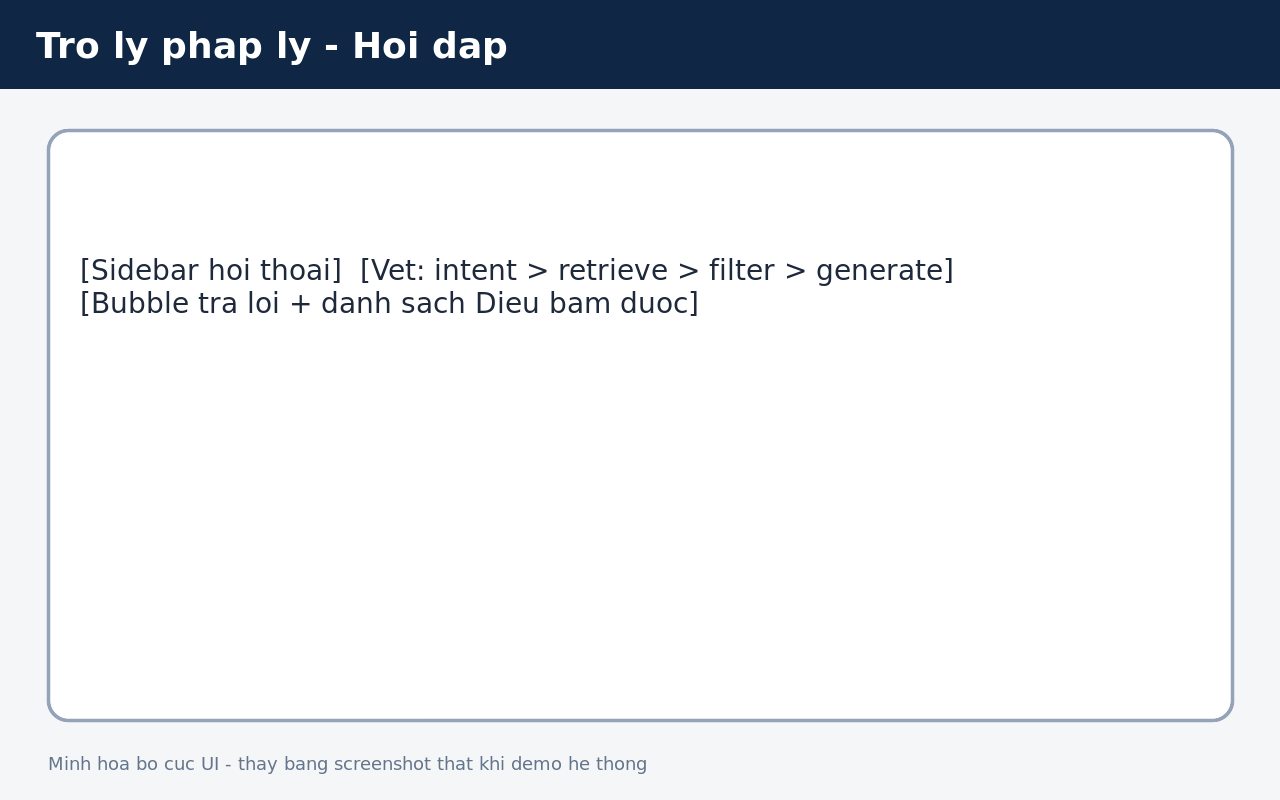
\includegraphics[width=0.88\linewidth]{man-hinh-chat.png}
\caption{Bố cục trang hỏi đáp: cột hội thoại, vết pipeline, câu trả lời và citation.}
\label{fig:man-hinh-chat}
\end{figure}

\begin{figure}[htp]
\centering
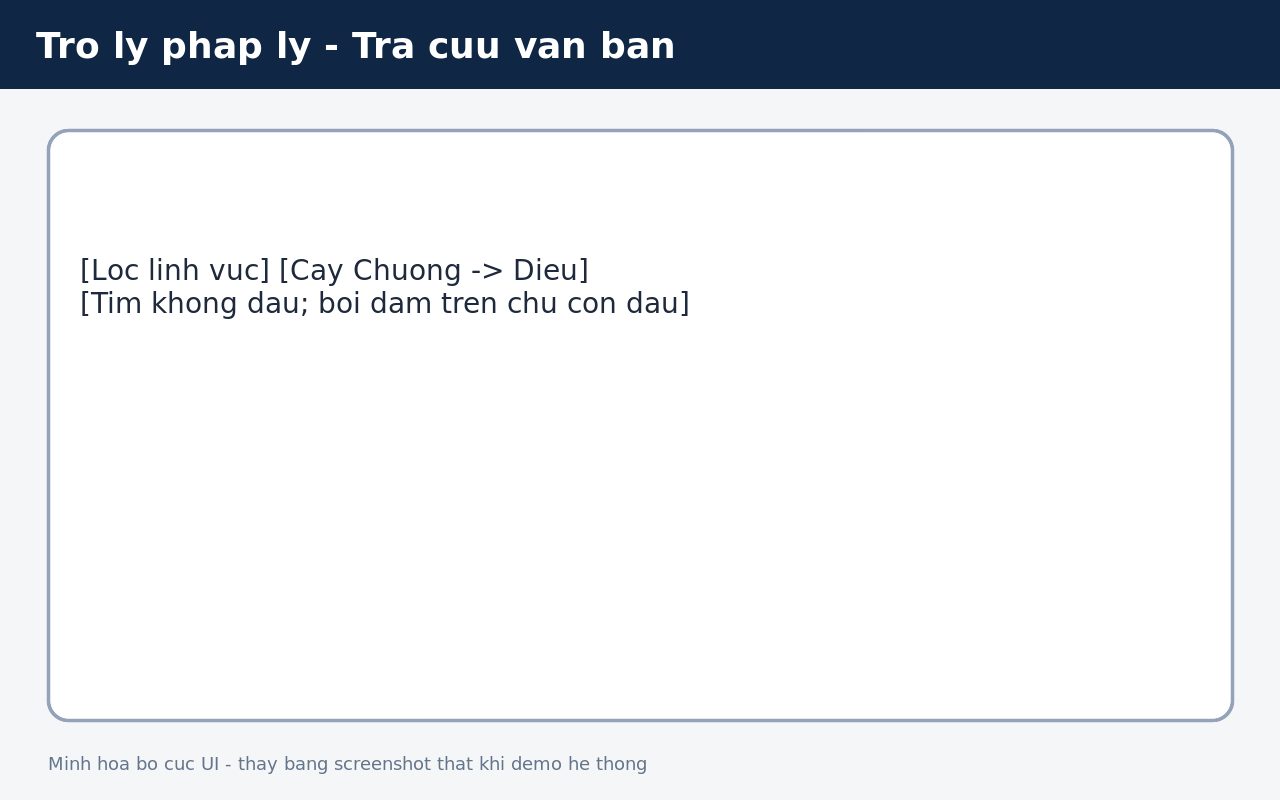
\includegraphics[width=0.88\linewidth]{man-hinh-tra-cuu.png}
\caption{Bố cục trang tra cứu: cây Chương--Điều và tìm không dấu.}
\label{fig:man-hinh-tra-cuu}
\end{figure}

\begin{figure}[htp]
\centering
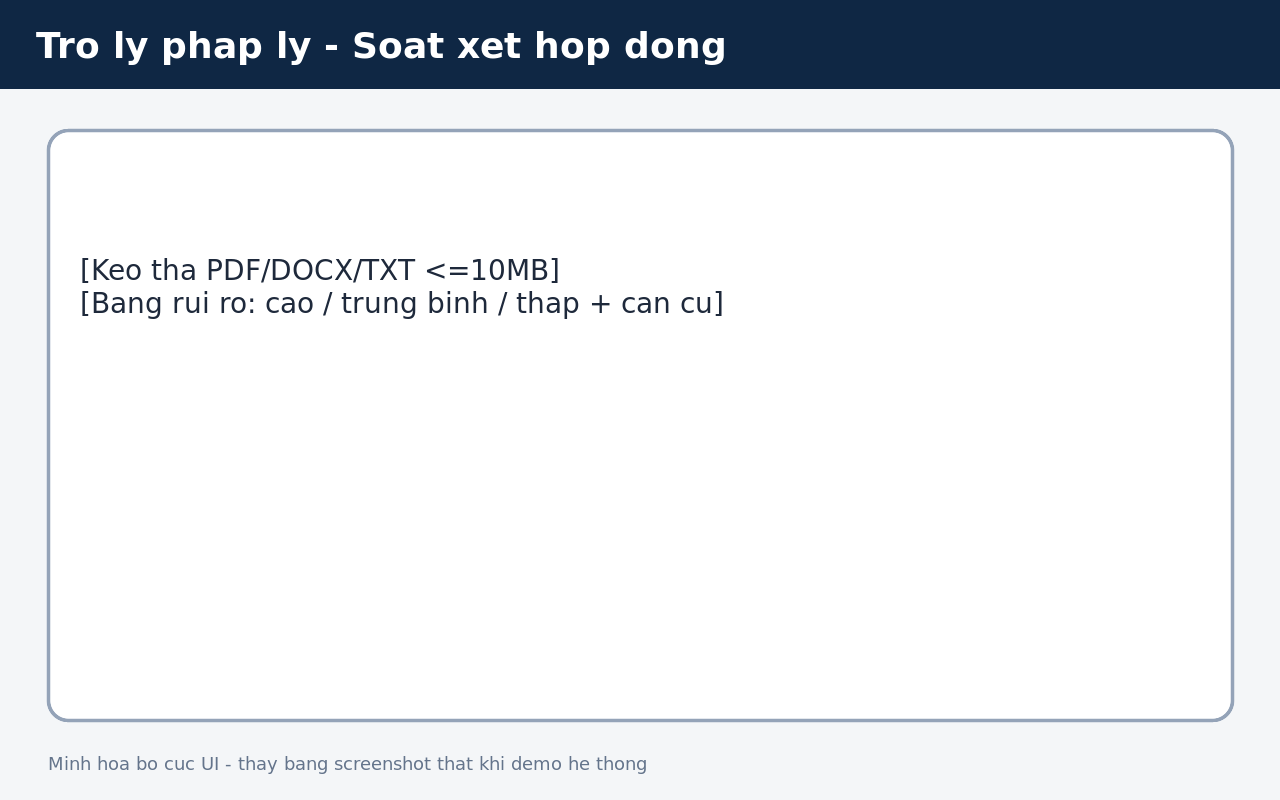
\includegraphics[width=0.88\linewidth]{man-hinh-hop-dong.png}
\caption{Bố cục trang hợp đồng: upload và bảng rủi ro.}
\label{fig:man-hinh-hop-dong}
\end{figure}

\begin{figure}[htp]
\centering
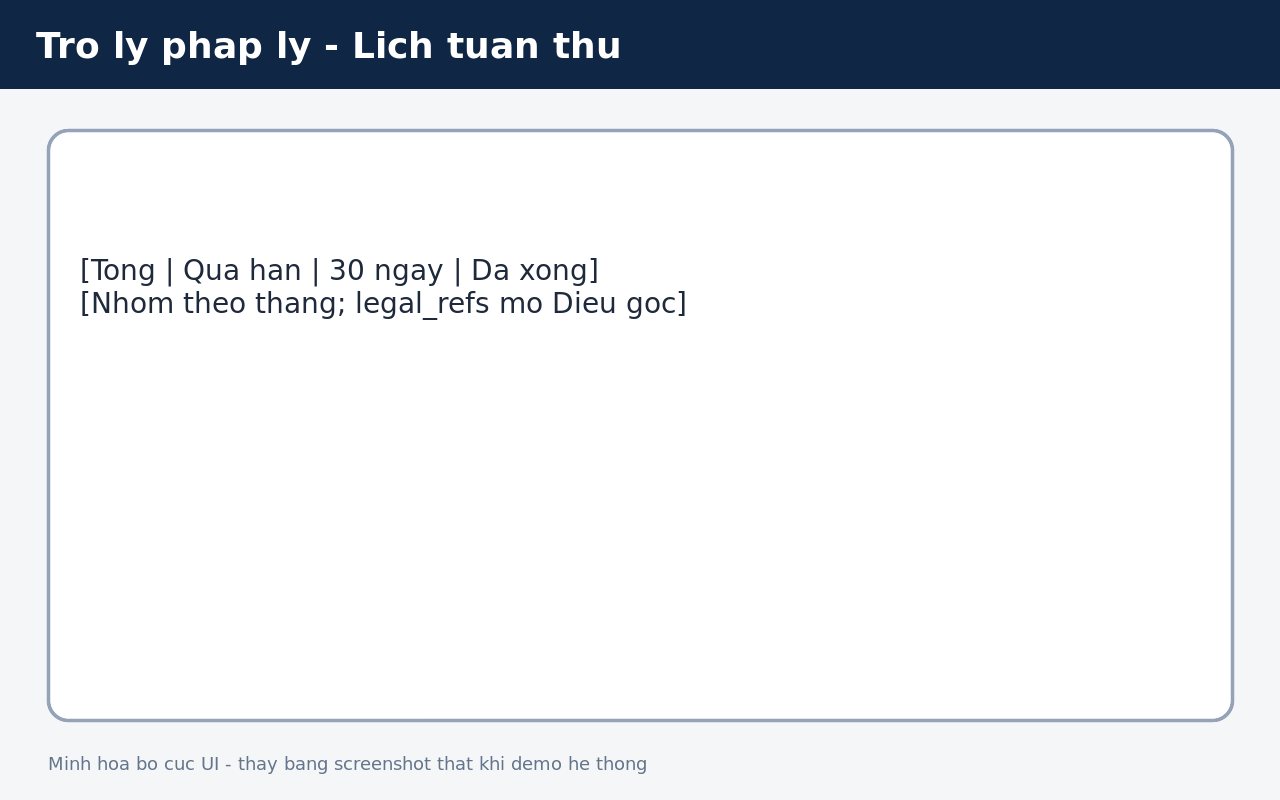
\includegraphics[width=0.88\linewidth]{man-hinh-lich.png}
\caption{Bố cục trang lịch tuân thủ: ô đếm và nhóm theo tháng.}
\label{fig:man-hinh-lich}
\end{figure}

Khi vận hành thử, cột vết pipeline giúp theo dõi tiến độ; nút ``Hỏi AI về Điều này'' trên trang luật hỗ trợ chuyển từ tra cứu sang hỏi đáp. Trên màn hẹp, thanh hội thoại còn chật --- đây là hạn chế giao diện.

\section{Đối chiếu mục tiêu Chương 1}

\begin{table}[htp]
\centering
\caption{Đối chiếu bảy mục tiêu cụ thể với bằng chứng.}
\label{tab:doi-chieu-mt}
\begin{tabular}{p{0.8cm}p{5.5cm}p{7.5cm}}
\toprule
\textbf{MT} & \textbf{Nội dung rút gọn} & \textbf{Bằng chứng} \\
\midrule
1 & Corpus cắt theo Điều & \soDieu{} bản ghi, manifest \soLuat{} luật \\
2 & Pipeline 7 bước + SSE & LangGraph + vết tiến độ trên UI \\
3 & Tra cứu cây + không dấu & 73 hit ``thue gtgt'' \\
4 & Soát xét hợp đồng nền & Upload 201, poll status \\
5 & Lịch \soRule{} rule & 39 task với hồ sơ mẫu \\
6 & JWT + cách ly & 404 khi xem chéo hội thoại \\
7 & Đóng gói Docker & Compose 3 dịch vụ \\
\bottomrule
\end{tabular}
\end{table}

\section{Tiêu chí đánh giá định tính}

Đánh giá sản phẩm khi chạy tay trên Compose theo năm tiêu chí (Bảng~\ref{tab:ket-qua-test}):

\begin{enumerate}
    \item Dẫn chiếu mở được Điều trong kho, không phải URL ngoại vi bịa.
    \item Tra cứu không dấu vẫn đọc được đoạn còn dấu.
    \item Suy giảm: thiếu LLM vẫn đăng nhập, đọc luật, xem lịch.
    \item Docker một lệnh cho ra đủ ba dịch vụ.
    \item Lịch khớp hồ sơ (quý/tháng, có/không lao động).
\end{enumerate}

Không tự gắn sao 1--5. Kết luận đạt/không đạt theo quan sát trên máy làm đồ án.

\subsection{Độ trễ, sẵn sàng và giới hạn đo}

\boncau
{Quan sát tay: FTS dưới một giây; hỏi đáp vài giây đến hơn mười giây (mạng
Gemini + HyDE + filter); soát xét vài trang chạy nền, poll 2,5 giây.}
{Chứng minh UI không đóng sớm và cụm vẫn sống khi thiếu khóa --- không phải
benchmark công bố.}
{Cố ý không gắn khóa: \texttt{/health} 200, login được, \texttt{GET /laws} đủ
\soLuat{} văn bản, FTS và lịch chạy; chỉ chat/soát xét 503 hoặc failed.}
{Không công bố ``trung bình $x$ giây'' (Wi-Fi, hạn mức miễn phí nhiễu). Không
công bố P/R/$F_2$: chưa gắn nhãn bộ câu nội bộ.}

\section{Kịch bản demo đề xuất khi bảo vệ}

Thứ tự dưới đây phủ đủ bốn nghiệp vụ và một nhánh lỗi:

\begin{enumerate}
    \item Đăng ký doanh nghiệp 12 lao động, GTGT quý; mở lịch, chỉ rule khớp.
    \item Tra cứu ``thue gtgt'' không dấu; mở một Điều; bấm hỏi về Điều đó.
    \item Đặt câu ``thử việc được bao lâu''; chỉ citation; đối chiếu Điều gốc.
    \item Tải \texttt{hd.txt}; đợi soát xét; đọc một finding.
    \item (Nếu có) tắt khóa hoặc xoá index tạm --- hỏi đáp 503, tra cứu còn.
\end{enumerate}

Kịch bản nhằm chứng minh hệ thống là ứng dụng vận hành được, không phải notebook RAG.


\chapter{Kết luận và hướng phát triển}

\section{Kết quả đạt được}

Đồ án đã xây dựng ứng dụng web chạy trên Docker Compose, hỗ trợ nhiều tài khoản
và nhiều tổ chức. Người dùng đặt câu hỏi tiếng Việt thông thường, nhận câu trả
lời kèm danh sách Điều mở được nguyên văn. Kho \soLuat{} văn bản được duyệt theo
cây Chương--Điều và tìm được khi thiếu dấu. Chức năng soát xét hợp đồng xuất bảng
rủi ro khi có khóa mô hình. Lịch tuân thủ sinh các mốc thuế, bảo hiểm, lao động
và BCTC theo hồ sơ từng doanh nghiệp.

Các quyết định kỹ thuật then chốt gồm: cắt ngữ liệu theo Điều; truy hồi lai BM25
và vector; hậu kiểm căn cứ so với tập truy hồi; tách pha tìm không dấu và pha
hiển thị còn dấu; dùng cột \texttt{seq} cho thứ tự tin nhắn; trả 404 khi truy cập
chéo hội thoại; duy trì đăng nhập và tra cứu khi thiếu khóa API.

Tầng máy chủ chạy trên PostgreSQL.

Đối chiếu bảy mục tiêu cụ thể ở Chương~1: corpus cắt theo Điều đạt ở mức nhập
và hiển thị, chưa đạt lịch sử hiệu lực; pipeline bảy bước và SSE đạt trên cấu
hình sản phẩm (nút rerank tắt); tra cứu cây và không dấu đạt; soát hợp đồng đạt
với tệp có lớp chữ; lịch \soRule{} rule đạt, công thức nằm trong mã; JWT và
cách ly đạt; Docker Compose đạt trên môi trường báo cáo. Mục tiêu ``mọi căn cứ
mở được Điều'' đạt khi kho đã nạp và citation đi qua hậu kiểm. Điều kiện đó
không biến câu chữ thành tư vấn pháp lý có chữ ký.

Ba chỗ dễ sai đã xử lý trong mã: không tin \texttt{created\_at} để sắp tin nhắn
trong cùng một giao dịch; Compose không đọc \texttt{backend/.env}; cùng origin
lúc đóng gói làm CORS gần như không chạy --- không sao chép \texttt{*} từ máy
lập trình sang máy thật.

\section{Hạn chế}

Đồ án không thực hiện OCR: tệp PDF ảnh bị từ chối lúc tải. Không dùng hàng đợi
phân tán. Không tự chọn bản luật còn hiệu lực khi hai số hiệu trùng tên khác năm.
Chưa đo P/R/F2 trên bộ câu gắn nhãn nội bộ. Giao diện chưa tối ưu cho điện thoại.
Token lưu tại \texttt{localStorage}.

Hậu kiểm chỉ đối chiếu số Điều, không phát hiện diễn giải sai trên Điều đúng.
HyDE và lọc LLM tiêu tốn hạn mức dịch vụ; nhúng lại toàn bộ \soDieu{} Điều trên
gói miễn phí dễ gặp mã 429, nên việc nhúng được chia lô và nghỉ dần.

\section{Hướng phát triển}

\begin{enumerate}
    \item Bổ sung OCR trước khi trích chữ, hoặc từ chối rõ ràng đối với PDF ảnh.
    \item Lưu ngày ban hành và hết hiệu lực trên từng Điều, lọc khi truy hồi.
    \item Gắn nhãn bộ câu nội bộ và đo P/R/F2 trên cùng corpus.
    \item Chuyển soát xét hợp đồng sang tiến trình worker riêng khi tệp dài.
    \item Mô hình hóa viện dẫn chéo thành đồ thị phục vụ câu hỏi đa văn bản.
    \item Chuyển token sang cookie \texttt{HttpOnly}, bổ sung CSP.
    \item Tối ưu giao diện cho màn hình hẹp.
\end{enumerate}

\section{Kết luận}

Đồ án giải quyết bài toán hỗ trợ DNNVV tra cứu và hỏi đáp pháp lý trong một kho
văn bản hẹp. Bốn nghiệp vụ --- hỏi đáp có nguồn, đọc cây văn bản, soát xét hợp
đồng, nhắc mốc tuân thủ --- chạy trên cùng một ứng dụng web đa người dùng. Hệ
thống không bao phủ mọi lĩnh vực pháp luật và không thay thế người hành nghề.
Nếu người dùng mở được Điều gốc trước khi hành động, sản phẩm đã đáp ứng mục
tiêu đã đặt ra.

\clearpage
\phantomsection
\addcontentsline{toc}{chapter}{TÀI LIỆU THAM KHẢO}
\begin{thebibliography}{99}

\bibitem{thanh2024}
Dương Hữu Thành, \textit{Công nghệ phần mềm}, NXB Thông tin và Truyền thông, 2024.

\bibitem{duong2026}
H. T. Duong, T. P. Bui, D. H. Nguyen, ``QLoRA and RAG Application in Building
Admissions Support Chatbot: Performance Evaluation and Knowledge Update
Ability,'' in N. N. Dao, V. Truong Hoang, F. Dornaika (eds.),
\textit{Explainable Intelligence in Digital Twins}, EIDT 2025, LNEE vol.~1531,
Springer, Singapore, 2026.

\bibitem{lewis2020rag}
P. Lewis, E. Perez, A. Piktus \textit{et al.}, ``Retrieval-Augmented Generation
for Knowledge-Intensive NLP Tasks,'' \textit{NeurIPS}, vol.~33, pp.~9459--9474,
2020.

\bibitem{karpukhin2020dpr}
V. Karpukhin, B. Oğuz, S. Min \textit{et al.}, ``Dense Passage Retrieval for
Open-Domain Question Answering,'' \textit{Proc. EMNLP}, pp.~6769--6781, 2020.

\bibitem{robertson2009bm25}
S. Robertson, H. Zaragoza, ``The Probabilistic Relevance Framework: BM25 and
Beyond,'' \textit{Foundations and Trends in Information Retrieval}, vol.~3,
no.~4, pp.~333--389, 2009.

\bibitem{cormack2009rrf}
G. V. Cormack, C. L. A. Clarke, S. Buettcher, ``Reciprocal Rank Fusion
Outperforms Condorcet and Individual Rank Learning Methods,'' \textit{Proc.
SIGIR}, pp.~758--759, 2009.

\bibitem{gao2023hyde}
L. Gao, X. Ma, J. Lin, J. Callan, ``Precise Zero-Shot Dense Retrieval without
Relevance Labels,'' \textit{Proc. ACL}, pp.~1762--1777, 2023.

\bibitem{quochoi2017}
Quốc hội, \textit{Luật Hỗ trợ doanh nghiệp nhỏ và vừa}, số 04/2017/QH14.

\bibitem{bll2019}
Quốc hội, \textit{Bộ luật Lao động}, số 45/2019/QH14.

\bibitem{qlthue2019}
Quốc hội, \textit{Luật Quản lý thuế}, số 38/2019/QH14.

\bibitem{postgresqlfts}
PostgreSQL Global Development Group, ``Full Text Search,'' tài liệu trực tuyến,
\url{https://www.postgresql.org/docs/current/textsearch.html}.

\bibitem{rfc7519}
M. Jones, J. Bradley, N. Sakimura, ``JSON Web Token (JWT),'' RFC~7519, 2015.

\bibitem{fastapi}
S. Ramírez, \textit{FastAPI documentation}, tài liệu trực tuyến,
\url{https://fastapi.tiangolo.com}.

\bibitem{react}
Meta, \textit{React documentation}, tài liệu trực tuyến,
\url{https://react.dev}.

\bibitem{docker}
Docker Inc., \textit{Docker documentation}, tài liệu trực tuyến,
\url{https://docs.docker.com}.

\bibitem{chromadb}
Chroma, \textit{Chroma documentation}, tài liệu trực tuyến,
\url{https://docs.trychroma.com}.

\bibitem{rfc9110}
R. Fielding, M. Nottingham, J. Reschke, ``HTTP Semantics,'' RFC~9110, 2022.

\bibitem{rfc8259}
T. Bray, ``The JavaScript Object Notation (JSON) Data Interchange Format,''
RFC~8259, 2017.

\bibitem{vaswani2017}
A. Vaswani, N. Shazeer, N. Parmar \textit{et al.}, ``Attention Is All You Need,''
\textit{NeurIPS}, 2017.

\bibitem{argon2}
A. Biryukov, D. Dinu, D. Khovratovich, ``Argon2: the memory-hard function for
password hashing and other applications,'' winner of the Password Hashing
Competition, 2015.

\bibitem{pdt590}
pdt590, ``vietnamese-legal-documents,'' Hugging Face Datasets, 2024.
\url{https://huggingface.co/datasets/pdt590/vietnamese-legal-documents}.

\end{thebibliography}

\clearpage
\phantomsection
\addcontentsline{toc}{chapter}{PHỤ LỤC}
\chapter*{PHỤ LỤC}

\section*{Phụ lục A. Chạy hệ thống trên máy}

Sao \texttt{.env.example} thành \texttt{.env} \textbf{ở thư mục gốc dự án},
không phải trong \texttt{backend/}. Compose không đọc \texttt{backend/.env}.
Điền \texttt{LLM\_API\_KEY} (trang AI Studio của Google) và
\texttt{JWT\_SECRET\_KEY} (ví dụ \texttt{openssl rand -hex 32}). Chạy:

\texttt{docker compose up -d --build}

Lần đầu nạp luật:

\texttt{docker compose exec backend python scripts/load\_postgres.py}
\texttt{--truncate}

Rồi restart backend. Vào \texttt{http://localhost:5173}. Tài khoản đăng ký đầu
tiên thành quản trị. Tra cứu dùng được ngay. Hỏi đáp cần đã nhúng vector: vào
\texttt{/admin/corpus} bấm reindex, hoặc đợi startup nếu khóa đã có từ đầu.

Thiếu khóa: web vẫn mở, hỏi đáp trả 503 chữ tiếng Việt, không phải stack trace.

\section*{Phụ lục B. Một số đường API}

\begin{longtable}{p{6.6cm}p{7.2cm}}
\toprule
\textbf{Đường} & \textbf{Việc} \\
\midrule
\endfirsthead
\toprule
\textbf{Đường} & \textbf{Việc} \\
\midrule
\endhead
\texttt{POST /api/v1/auth/register} & Tạo user, có thể kèm organization \\
\texttt{POST /api/v1/auth/login} & Cấp access + refresh \\
\texttt{POST /api/v1/auth/refresh} & Đổi access, kiểm tra \texttt{type} \\
\texttt{GET /api/v1/conversations} & Danh sách hội thoại của đúng user \\
\texttt{POST /api/v1/legal/chat/stream} & SSE hỏi đáp \\
\texttt{GET /api/v1/laws} & Catalog \\
\texttt{GET /api/v1/laws/search} & FTS \\
\texttt{GET /api/v1/laws/\{id\}/articles} & Cây Chương--Điều \\
\texttt{POST /api/v1/documents} & Tải file \\
\texttt{POST /api/v1/documents/\{id\}/review} & 202, chạy nền \\
\texttt{GET /api/v1/compliance/tasks} & Lịch \\
\texttt{POST /api/v1/admin/corpus/reindex} & Nhúng lại, chỉ admin \\
\bottomrule
\end{longtable}

\section*{Phụ lục C. Chạy hàng loạt câu hỏi}

Quản trị mở trang \texttt{/admin/batch-eval}, gửi một mảng JSON (mỗi phần tử có
câu hỏi) để pipeline chạy lần lượt, xem tiến độ và tải kết quả. Chế độ này bỏ
qua phân tích ý định (luôn truy hồi) và không gắn lịch sử hội thoại, nhằm tái
lập được trên cùng bộ câu. User thường không gọi được các đường này.

\section*{Phụ lục D. Ghi chú biên dịch báo cáo}

File \texttt{main.tex} phải chạy XeLaTeX (gói \texttt{fontspec}). Trong Cursor
hoặc VS Code, biên dịch bằng recipe xelatex (hoặc \texttt{latexmk -xelatex}).
Đầu file có chỉ thị TEX program trỏ sang xelatex. Ảnh minh họa nằm trong thư mục
\texttt{Baocao/images/}; không dùng tùy chọn \texttt{demo} của \texttt{graphicx}
(tùy chọn đó vẽ hình đen đặc).

\section*{Phụ lục E. Biến môi trường chính}

\begin{longtable}{p{5.2cm}p{8.6cm}}
\toprule
\textbf{Biến} & \textbf{Ý nghĩa} \\
\midrule
\endfirsthead
\toprule
\textbf{Biến} & \textbf{Ý nghĩa} \\
\midrule
\endhead
\texttt{LLM\_API\_KEY} & Khóa gọi Gemini (sinh câu) \\
\texttt{EMBEDDINGS\_API\_KEY} & Khóa nhúng; có thể trùng khóa LLM \\
\texttt{JWT\_SECRET\_KEY} & Khóa ký JWT, tối thiểu đủ dài ngẫu nhiên \\
\texttt{LEGAL\_DATABASE\_URL} & Chuỗi kết nối Postgres (Compose tự ghép) \\
\texttt{CORS\_ALLOW\_ORIGINS} & Danh sách origin, dùng lúc dev Vite \\
\texttt{LLM\_MODEL} & Mặc định \texttt{gemini-2.5-flash} \\
\texttt{EMBEDDINGS\_MODEL} & Mặc định \texttt{gemini-embedding-001} \\
\texttt{POSTGRES\_PORT} & Mặc định 23432 trên host \\
\bottomrule
\end{longtable}

\section*{Phụ lục F. Cấu trúc thư mục mã nguồn}

\begin{itemize}
    \item \path{backend/src/routers}: cổng HTTP.
    \item \path{backend/src/services/agents}: LangGraph.
    \item \path{backend/src/services/vector_store}: BM25, Chroma, hybrid.
    \item \path{backend/src/services/legal}: FTS, catalog.
    \item \path{backend/src/services/contracts}: trích chữ, soát xét.
    \item \path{backend/src/services/compliance}: seed và sinh lịch.
    \item \path{backend/src/models}: ORM.
    \item \path{backend/alembic}: migration.
    \item \path{frontend/src/pages}: trang.
    \item \path{frontend/src/components/chat}: hội thoại.
    \item \path{corpus/law_manifest.json}: danh mục số hiệu.
    \item \path{data/base_data.json}: Điều.
    \item \path{Baocao/}: nguồn báo cáo XeLaTeX.
\end{itemize}

\section*{Phụ lục G. Use case còn lại (rút gọn)}

UC-01: khách gửi email, mật khẩu, hồ sơ công ty; hệ thống tạo user, có thể gắn
admin nếu là người đầu; sinh lịch nếu có tổ chức. UC-02: login cấp hai token;
refresh đổi access. UC-04: đổi tên hội thoại, xóa mềm hoặc xóa hẳn tùy API; không
xem hội thoại người khác. UC-06: ô tìm trên \texttt{/laws}, ba tầng FTS. UC-08:
thành viên cùng tổ chức xem finding. UC-10: admin import JSON, reindex. UC-11:
admin khóa tài khoản hoặc đổi vai trò. UC-12: admin gửi bộ câu, nhận file kết quả.

\section*{Phụ lục H. Thuật ngữ gắn với cách đóng gói đồ án}

\textbf{Container} ở đây là một trong ba tiến trình Compose (Postgres, backend,
nginx). \textbf{Image} là bản đóng gói từng dịch vụ. \textbf{Volume}
\texttt{postgres\_data}, \texttt{chroma\_db}, \texttt{uploads} giữ dữ liệu khi
tắt cụm. \textbf{Proxy} là nginx nhận một cổng rồi chuyển \texttt{/api} vào
backend. \textbf{Healthcheck} là \texttt{pg\_isready} và \texttt{/health}, để
backend đợi CSDL sẵn sàng. \textbf{Migration} là bản Alembic đổi cột.
\textbf{Interceptor} là hàm Axios gắn token và gỡ JSON khi gửi file.
\textbf{Splat} là đoạn URL bắt phần còn lại, dùng cho số hiệu có dấu \texttt{/}.

\section*{Phụ lục I. Quy trình nạp corpus và lập chỉ mục}

Nạp chữ vào Postgres tách khỏi nhúng vector. \texttt{scripts/load\_postgres.py}
đọc JSON Điều, ghi \texttt{legal\_knowledge\_records} (tuỳ chọn
\texttt{--truncate}). Generated column tự tính số Điều và tsvector. Tra cứu dùng
ngay sau bước này, không cần khóa Gemini.

Nhúng: lúc khởi động hoặc khi quản trị bấm reindex, hệ thống đọc từng Điều, gọi
embedding theo lô 64 bản ghi, ghi vào Chroma, rồi ghi manifest (mô hình, số
chiều, số vector). Khác mô hình hoặc khác chiều so với
manifest: bắt buộc nhúng lại. Thiếu khóa: bỏ qua nhúng, \texttt{/health} vẫn 200.

BM25: tách từ, cache đĩa theo tokenizer. Không nhầm cache BM25 với volume
Chroma.

Thứ tự an toàn khi máy trắng: Compose up, đợi health, load\_postgres, restart
backend, (nếu có khóa) reindex trên admin. Đảo thứ tự (reindex trước khi có
hàng Postgres) cho chỉ mục rỗng hoặc lệch id.

\section*{Phụ lục J. Ràng buộc đạo đức và trách nhiệm sử dụng}

Hệ thống hỗ trợ thông tin trên kho đóng. Không thay thế luật sư, đại lý thuế,
hoặc cơ quan nhà nước. Người dùng phải mở Điều gốc trước khi hành động có hậu
quả pháp lý. Nhật ký hội thoại chứa câu hỏi doanh nghiệp --- triển khai thật
cần chính sách lưu trữ và quyền xóa (đồ án mới có xóa hội thoại theo chủ sở
hữu). Không thu thập dữ liệu cá nhân ngoài tài khoản thử nghiệm.






\end{document}
